\input{../utils/preamble}
\createdgmtitle{9}
%--------------------------------------------------------------------------------
\begin{document}
%--------------------------------------------------------------------------------
\begin{frame}
%\thispagestyle{empty}
\titlepage
\end{frame}
%=======
\begin{frame}{Recap of previous lecture}
	\begin{block}{ELBO surgery}
	\vspace{-0.6cm}
	\[
	    \frac{1}{n} \sum_{i=1}^n \cL_i(q, \btheta) = \underbrace{\frac{1}{n} \sum_{i=1}^n \mathbb{E}_{q(\bz | \bx_i)} \log p(\bx_i | \bz, \btheta)}_{\text{Reconstruction loss}}
	    - \underbrace{\vphantom{ \sum_{i=1}^n} \bbI_q [\bx, \bz]}_{\text{MI}} - \underbrace{\vphantom{ \sum_{i=1}^n} KL(q(\bz) || p(\bz))}_{\text{Marginal KL}}
	\]
	\end{block}
	\vspace{-0.8cm}
	\begin{block}{Optimal prior}
		\vspace{-0.4cm}
		\[
		KL(q(\bz) || p(\bz)) = 0 \quad \Leftrightarrow \quad p (\bz) = q(\bz) = \frac{1}{n} \sum_{i=1}^n q(\bz | \bx_i).
		\]
		\vspace{-0.2cm}\\
		The optimal prior distribution $p(\bz)$ is aggregated posterior $q(\bz)$.
	\end{block}

	\begin{block}{VampPrior}
		\vspace{-0.4cm}
		\[
		p(\bz | \blambda) = \frac{1}{K} \sum_{k=1}^K q(\bz | \bu_k),
		\]
		\vspace{-0.2cm} \\
		where $\blambda = \{\bu_1, \dots, \bu_K\}$ are trainable pseudo-inputs.
	\end{block}
	\myfootnotewithlink{https://arxiv.org/abs/1705.07120}{Tomczak J. M., Welling M. VAE with a VampPrior, 2017}
\end{frame}
%=======
\begin{frame}{Recap of previous lecture}
	\begin{block}{Autoregressive flow prior}
		\vspace{-0.5cm}
		\[
			\log p(\bz | \blambda) = \log p(\bepsilon) + \log \det \left | \frac{d \bepsilon}{d\bz}\right|; \quad 
			\bz = g(\bepsilon, \blambda) = f^{-1}(\bepsilon, \blambda)
		\]
	\end{block}
	\vspace{-0.4cm}
	\begin{block}{Theorem}
	VAE with the AF prior for latent code $\bz$ is equivalent to using the IAF posterior for latent code $\bepsilon$.
	\end{block}
	{\footnotesize
	\begin{align*}
		\mathcal{L}(q, \btheta) &= \mathbb{E}_{\bz \sim q(\bz | \bx)} \Bigl[ \log p(\bx | \bz, \btheta) + \underbrace{ \Bigl( \log p(f(\bz, \blambda)) + \log \left| \det \frac{\partial f(\bz, \blambda)}{\partial \bz} \right| \Bigr) }_{\text{AF prior}} - \log q(\bz | \bx) \Bigr] \\
		&= \mathbb{E}_{\bz \sim q(\bz | \bx)} \Bigl[ \log p(\bx | \bz, \btheta) +  \log p(f(\bz, \blambda)) - \underbrace{ \Bigl( \log q(\bz | \bx) - \log \left| \det \frac{\partial f(\bz, \blambda)}{\partial \bz} \right| \Bigr) }_{\text{IAF posterior}} \Bigr]
	\end{align*}
	}
	\myfootnotewithlink{https://arxiv.org/abs/1611.02731}{Chen X. et al. Variational Lossy Autoencoder, 2016}
\end{frame}
%=======
\begin{frame}{Recap of previous lecture}
	\begin{block}{LVM}
		\vspace{-0.3cm}
		\[
		    p(\bx | \btheta) = \int p(\bx, \bz | \btheta) d \bz = \int p(\bx | \bz, \btheta) p(\bz) d \bz 
		\]
		\vspace{-0.3cm}
	\end{block}
	\begin{itemize}
		\item More powerful $p(\bx | \bz, \btheta)$ leads to more powerful generative model $p(\bx | \btheta)$.
		\item Too powerful $p(\bx | \bz, \btheta)$ could lead to posterior collapse: $q(\bz | \bx)$ will not carry any information about $\bx$ and close to prior $p(\bz)$.
	\end{itemize}
	\begin{block}{Autoregressive decoder}
		\vspace{-0.2cm}
		\[
		    p(\bx | \bz , \btheta) = \prod_{i=1}^n p(x_i | \bx_{1:i - 1}, \bz , \btheta)
		\]
	\end{block}
	\begin{itemize}
		\item Global structure is captured by latent variables.
		\item Local statistics are captured by limited receptive field autoregressive model.
	\end{itemize}
	
	\myfootnotewithlink{https://arxiv.org/abs/1611.05013}{Gulrajani I. et al. PixelVAE: A Latent Variable Model for Natural Images, 2016}
\end{frame}
%=======
\begin{frame}{Recap of previous lecture}
	\begin{block}{Decoder weakening}
		\begin{itemize}
			\item Powerful decoder $p(\bx | \bz, \btheta)$ makes the model expressive, but posterior collapse is possible.
			\item PixelVAE model uses the autoregressive PixelCNN model with small number of layers to limit receptive field.
		\end{itemize}
	\end{block}
	
	\begin{block}{KL annealing}
		\vspace{-0.2cm}
		\[
		    \mathcal{L}(q, \btheta, \beta) = \mathbb{E}_{q(\bz | \bx)} \log p(\bx | \bz, \btheta) - \beta \cdot KL (q(\bz | \bx) || p(\bz))
		\]
		Start training with $\beta = 0$, increase it until $\beta = 1$ during training.
	\end{block}
	
	\begin{block}{Free bits}
		Ensure the use of less than $\lambda$ bits of information:
		\[
		    \mathcal{L}(q, \btheta, \lambda) = \mathbb{E}_{q(\bz | \bx)} \log p(\bx | \bz, \btheta) - \max(\lambda, KL (q(\bz | \bx) || p(\bz))).
		\]
		This results in $KL (q(\bz | \bx) || p(\bz)) \geq \lambda$.
	\end{block}
\end{frame}
%=======
\begin{frame}{Recap of previous lecture}
	\begin{block}{Disentanglement learning}
	A disentangled representation is a one where single latent units are sensitive to changes in single generative factors, while being invariant to changes in other factors. 
	\end{block}
	\begin{block}{$\beta$-VAE}
	\vspace{-0.2cm}
	\[
	    \mathcal{L}(q, \btheta, \beta) = \mathbb{E}_{q(\bz | \bx)} \log p(\bx | \bz, \btheta) - \beta \cdot KL (q(\bz | \bx) || p(\bz)).
	\]
	Representations becomes disentangled by setting a stronger constraint with $\beta > 1$. However, it leads to poorer reconstructions and a loss of high frequency details. 
	\end{block}
	
	\begin{block}{ELBO surgery}
		\vspace{-0.3cm}
		{\footnotesize
			\[
			\frac{1}{n} \sum_{i=1}^n \cL_i(q, \btheta, \beta) = \underbrace{\frac{1}{n} \sum_{i=1}^n \mathbb{E}_{q(\bz | \bx_i)} \log p(\bx_i | \bz, \btheta)}_{\text{Reconstruction loss}} - \beta \cdot \underbrace{\bbI_{q} [\bx, \bz]\vphantom{\sum_{i=1}}}_{\text{MI}} - \beta \cdot \underbrace{KL(q(\bz) || p(\bz))\vphantom{\sum_{i=1}}}_{\text{Marginal KL}}
			\]}
	\end{block}
	\myfootnotewithlink{https://arxiv.org/abs/1804.03599}{Burgess C. P. et al. Understanding disentangling in $\beta$-VAE, 2018}
\end{frame}
%=======
\begin{frame}{DIP-VAE}
	\begin{block}{Disentangled aggregated variational posterior}
		\vspace{-0.3cm}
		\[
		q(\bz) = \frac{1}{n} \sum_{i=1}^n q(\bz | \bx) = \prod_{j=1}^d q(z_j)
		\]
		\vspace{-0.3cm}
	\end{block}
	\begin{block}{DIP-VAE Objective}
		\vspace{-0.3cm}
		{\footnotesize
			\begin{multline*}
			\cL_{\text{DIP}}(q, \btheta) = \frac{1}{n} \sum_{i=1}^n \cL_i(q, \btheta) -\lambda \cdot KL(q(\bz) || p(\bz)) = \\
			= \frac{1}{n} \sum_{i=1}^n\left[ \bbE_{q(\bz | \bx_i)} \log p(\bx_i | \bz, \btheta) - KL(q(\bz | \bx_i) || p(\bz)) \right] -\lambda \cdot KL(q(\bz) || p(\bz)) = \\
			= \underbrace{ \frac{1}{n} \sum_{i=1}^n \left[\bbE_{q(\bz | \bx_i)} \log p(\bx_i | \bz, \btheta)\right]}_{\text{Reconstruction loss}} - \underbrace{\vphantom{\sum_{i=1}^n} \bbI_{q} [\bx, \bz]}_{\text{MI}} - (1 + \lambda) \cdot \underbrace{\vphantom{\sum_{i=1}^n} KL(q(\bz) || p(\bz))}_{\text{Marginal KL}}
			\end{multline*}
		}
		\vspace{-0.3cm}
	\end{block}

	\myfootnotewithlink{https://arxiv.org/abs/1711.00848}{Kumar A., Sattigeri P., Balakrishnan A. Variational Inference of Disentangled Latent Concepts from Unlabeled Observations, 2017}
\end{frame}
%=======
\begin{frame}{DIP-VAE}
		\vspace{-0.2cm}
		\[
			\cL_{\text{DIP}}(q, \btheta) = \frac{1}{n} \sum_{i=1}^n \cL_i(q, \btheta) -\lambda \cdot \underbrace{KL(q(\bz) || p(\bz))}_{\text{intractable}}
		\]
	Let match the moments of $q(\bz)$ and $p(\bz)$:
	\[
	\text{cov}_{q(\bz)}(\bz) = \bbE_{q(\bz)} \left[ (\bz - \bbE_{q(\bz)}(\bz)) (\bz - \bbE_{q(\bz)}(\bz))^T \right]
	\]
	DIP-VAE regularizes $\text{cov}_{q(\bz)}(\bz) $ to be close to the identity matrix. 
	\begin{block}{Objective}
		\vspace{-0.5cm}
		\begin{multline*}
		\max_{q, \btheta} \Bigl[\frac{1}{n} \sum_{i=1}^n \cL_i(q, \btheta) - \\ - \lambda_1 \sum_{i \neq j} \left[\text{cov}_{q(\bz)} (\bz) \right]^2_{ij} - \lambda_2 \sum_{i} \left( \left[ \text{cov}_{q(\bz)} (\bz) \right]_{ii} - 1 \right)^2 \Bigr]
		\end{multline*}
		\vspace{-0.5cm}
	\end{block}

	\myfootnotewithlink{https://arxiv.org/abs/1711.00848}{Kumar A., Sattigeri P., Balakrishnan A. Variational Inference of Disentangled Latent Concepts from Unlabeled Observations, 2017}
\end{frame}
%=======
\begin{frame}{DIP-VAE}
	\begin{figure}
		\centering
		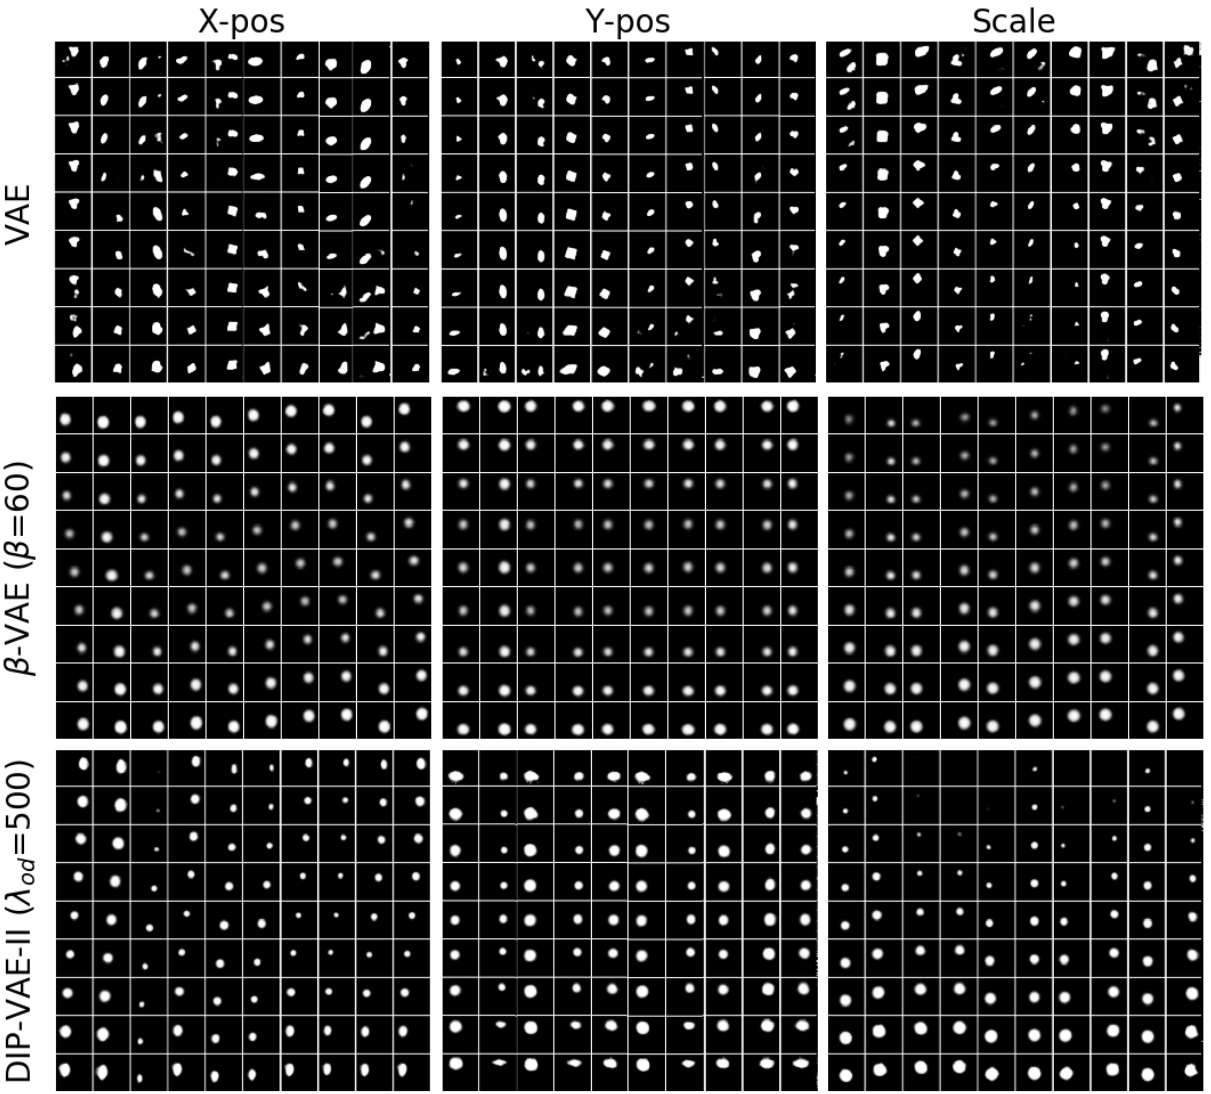
\includegraphics[width=0.75\linewidth]{figs/dip-vae_1}
	\end{figure}

	\myfootnotewithlink{https://arxiv.org/abs/1711.00848}{Kumar A., Sattigeri P., Balakrishnan A. Variational Inference of Disentangled Latent Concepts from Unlabeled Observations, 2017}
\end{frame}
%=======
\begin{frame}{DIP-VAE}
	\begin{figure}
		\centering
		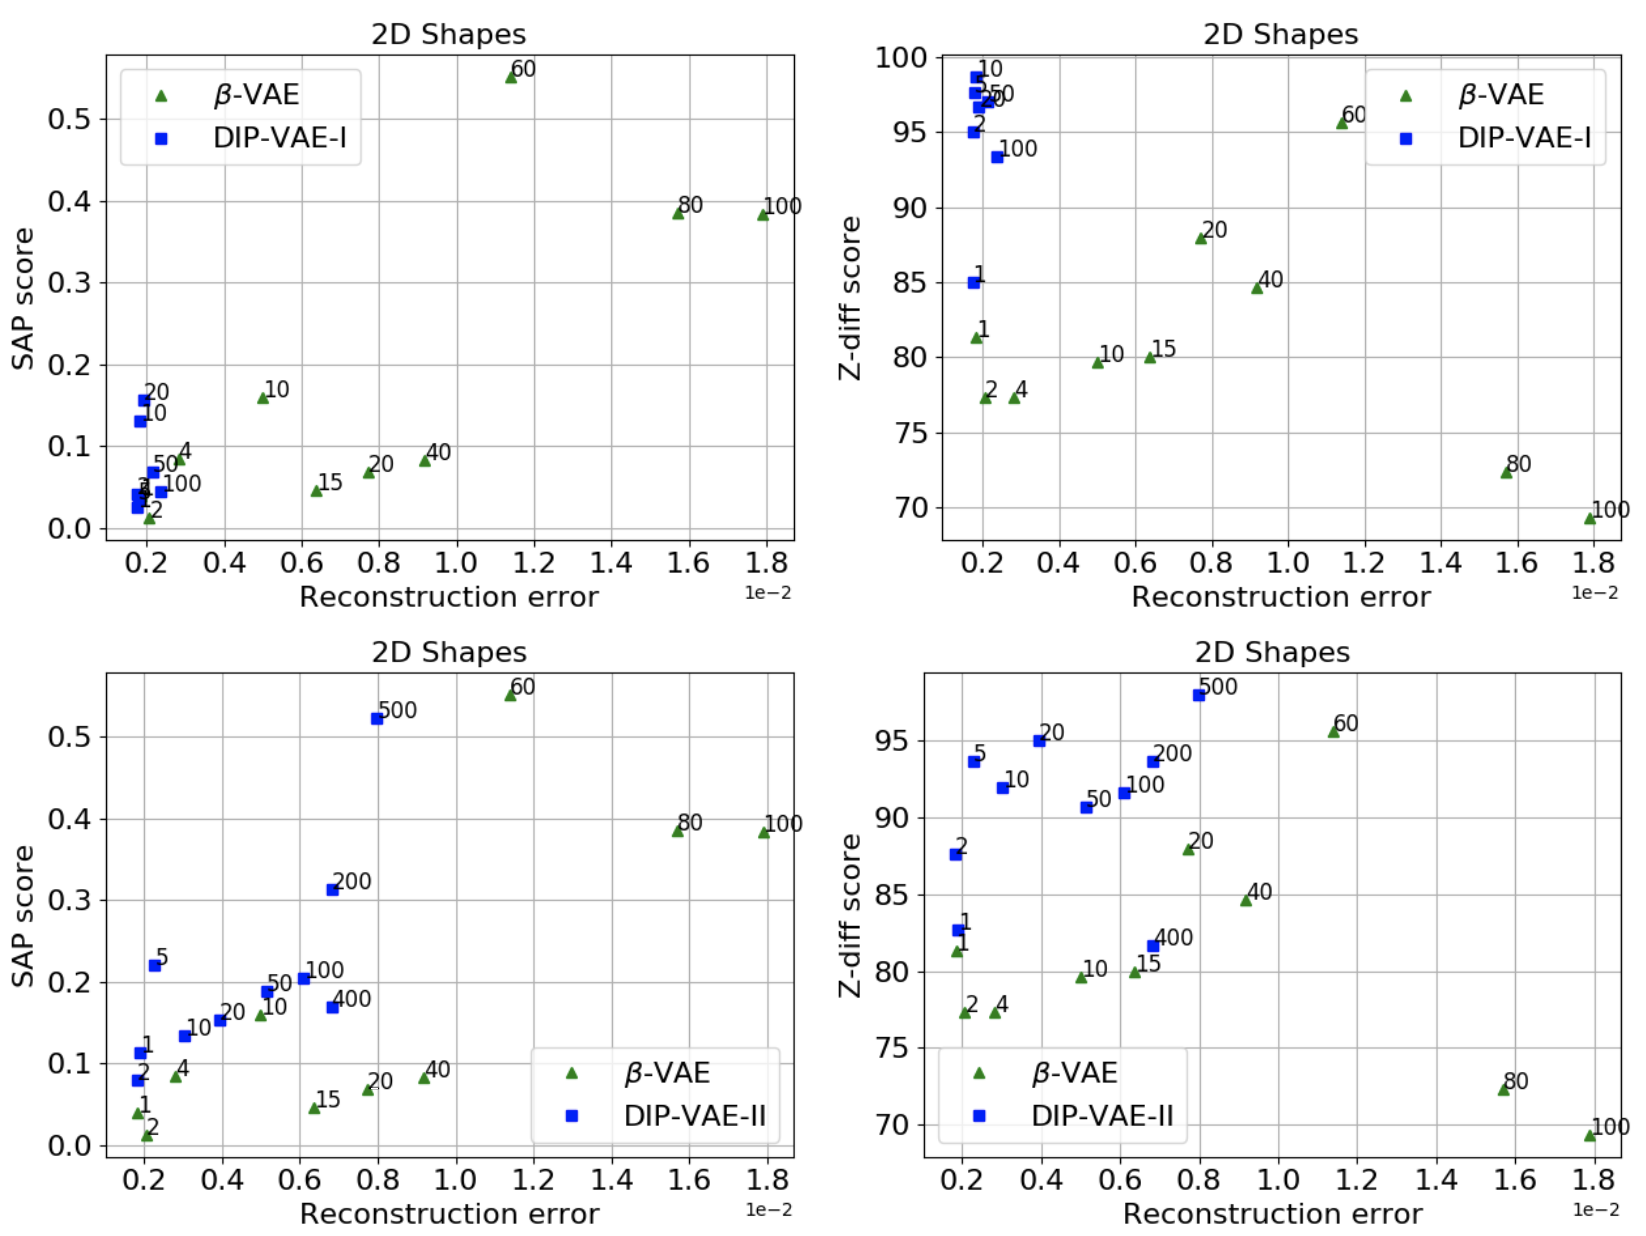
\includegraphics[width=0.9\linewidth]{figs/dip-vae_2}
	\end{figure}

	\myfootnotewithlink{https://arxiv.org/abs/1711.00848}{Kumar A., Sattigeri P., Balakrishnan A. Variational Inference of Disentangled Latent Concepts from Unlabeled Observations, 2017}
\end{frame}
%=======
\begin{frame}{Challenging Disentanglement Assumptions}
Whether unsupervised disentanglement learning is even possible for arbitrary generative models?

\begin{block}{Theorem}
	For $d > 1$, let $\bz \sim P$ denote any distribution which admits a density $p(\bz) = \prod^d_{i=1} p(z_i)$. Then, there exists an infinite family of bijective functions $f : \text{supp}(\bz) \rightarrow \text{supp}(\bz)$ such that
	\begin{itemize}
		\item $\frac{\partial f_i(\bu)}{\partial u_j} \neq 0$ almost everywhere for all $i$ and $j$ (i.e., $\bz$ and $f(\bz)$ are completely entangled);
		\item and $P(\bz \leq \bu) = P(f(\bz) \leq \bu)$ for all $\bu \in \text{supp}(\bz)$ (i.e., they
		have the same marginal distribution).
	\end{itemize}  
\end{block}

Theorem claims that unsupervised disentanglement learning is impossible for arbitrary generative models with a factorized prior.

\myfootnotewithlink{https://arxiv.org/abs/1811.12359}{Locatello F. et al. Challenging Common Assumptions in the Unsupervised Learning of Disentangled Representations, 2018}
\end{frame}
%=======
\begin{frame}{Challenging Disentanglement Assumptions}
Assume we have $p(\bz)$ and some $p(\bx|\bz)$ defining a generative model. Consider any unsupervised
disentanglement method and assume that it finds a representation that is perfectly disentangled with respect
to $\bz$ in the generative model.
\begin{itemize}
	\item Theorem claims that $\exists$ $\hat{\bz} = f(\bz)$ where $\hat{\bz}$ is completely entangled
	with respect to $\bz$.
	\item Since the (unsupervised) disentanglement method only has access to
	observations $\bx$, it hence cannot distinguish between the two equivalent generative models and thus has to be entangled to at least one of them
	\[
	p(\bx) = \int p(\bx | \bz) p(\bz) d\bz = \int p(\bx | \hat{\bz})p(\hat{\bz}) d \hat{\bz}.
	\]
\end{itemize}

\myfootnotewithlink{https://arxiv.org/abs/1811.12359}{Locatello F. et al. Challenging Common Assumptions in the Unsupervised Learning of Disentangled Representations, 2018}
\end{frame}
%=======
\begin{frame}{Challenging Disentanglement Assumptions}
\begin{block}{Proof (1)}
	\begin{enumerate}
		\item 
		Consider the function $g: \text{supp}(\bz) \rightarrow [0, 1]^d$:
		\vspace{-0.1cm}
		\[
		g_i(\bv) = P(z_i \leq v_i), \quad i=1, \dots, d.
		\]
		\vspace{-0.4cm}
		\begin{itemize}
			\item $g$ is bijective (since $p(\bz) = \prod_{i=1}^dp(z_i)$).
			\item $\frac{\partial g_i(\bu)}{\partial u_i} \neq 0$, for all $i$ and $\frac{\partial g_i(\bu)}{\partial u_j} = 0$ for all $i \neq j$.
			\item $g(\bz)$ is an independent $d$-dimensional uniform distribution.
		\end{itemize}
		\item 
		Consider $h: (0, 1]^d \rightarrow \bbR^d$
		\[
		h_i(\bv) = \psi^{-1}(v_i), \quad i= 1, \dots, d.
		\]
		Here $\psi$  denotes the CDF of a standard normal distribution.
		\begin{itemize}
			\item $h$ is bijective.
			\item $\frac{\partial g_i(\bu)}{\partial u_i} \neq 0$, for all $i$ and $\frac{\partial g_i(\bu)}{\partial u_j} = 0$ for all $i \neq j$.
			\item $h(g(\bz))$  is a $d$-dimensional standard normal distribution.
		\end{itemize}
	\end{enumerate}
\end{block}

\myfootnotewithlink{https://arxiv.org/abs/1811.12359}{Locatello F. et al. Challenging Common Assumptions in the Unsupervised Learning of Disentangled Representations, 2018}
\end{frame}
\begin{frame}{Challenging Disentanglement Assumptions}
\begin{block}{Proof (2)}
	Let $\bA \in \bbR^{d \times d}$ be an arbitrary orthogonal matrix with $A_{ij} \neq 0$ for all $i, j$.
	The family of such matrices is infinite.
	\begin{itemize}
		\item $\bA$ is orthogonal, it is invertible and thus defines a bijective linear operator. 
		\item $\bA h(g(\bz)) \in \bbR^d$ is hence an independent, multivariate standard normal distribution.
		\item $h^{-1}( \bA h(g(\bz))) \in \bbR^d$ is an independent $d$-dimensional uniform distribution.
	\end{itemize}
	Define $f: \text{supp}(\bz) \rightarrow \text{supp}(\bz)$:
	\vspace{-0.2cm}
	\[
	f(\bu) = g^{-1} (h^{-1}( \bA h(g(\bz)))).
	\]
	By definition $f(\bz)$ has the same marginal distribution as $\bz$: $P(\bz \leq \bu) = P(f(\bz) \leq \bu)$ and $\frac{\partial f_i(\bu)}{\partial u_j} \neq 0$.
\end{block}

\myfootnotewithlink{https://arxiv.org/abs/1811.12359}{Locatello F. et al. Challenging Common Assumptions in the Unsupervised Learning of Disentangled Representations, 2018}
\end{frame}
%=======
\begin{frame}{Challenging Disentanglement Assumptions}
\begin{itemize}
	\item \textbf{Training:} Factorizing \textbf{samples} from aggregated posterior $q(\bz) = \prod_{i=1}^d q(z_i)$.
	\item \textbf{Inference:} Use a \textbf{mean} vector (usually mean of Gaussian encoder) as a representation.
\end{itemize}
\begin{figure}
	\centering
	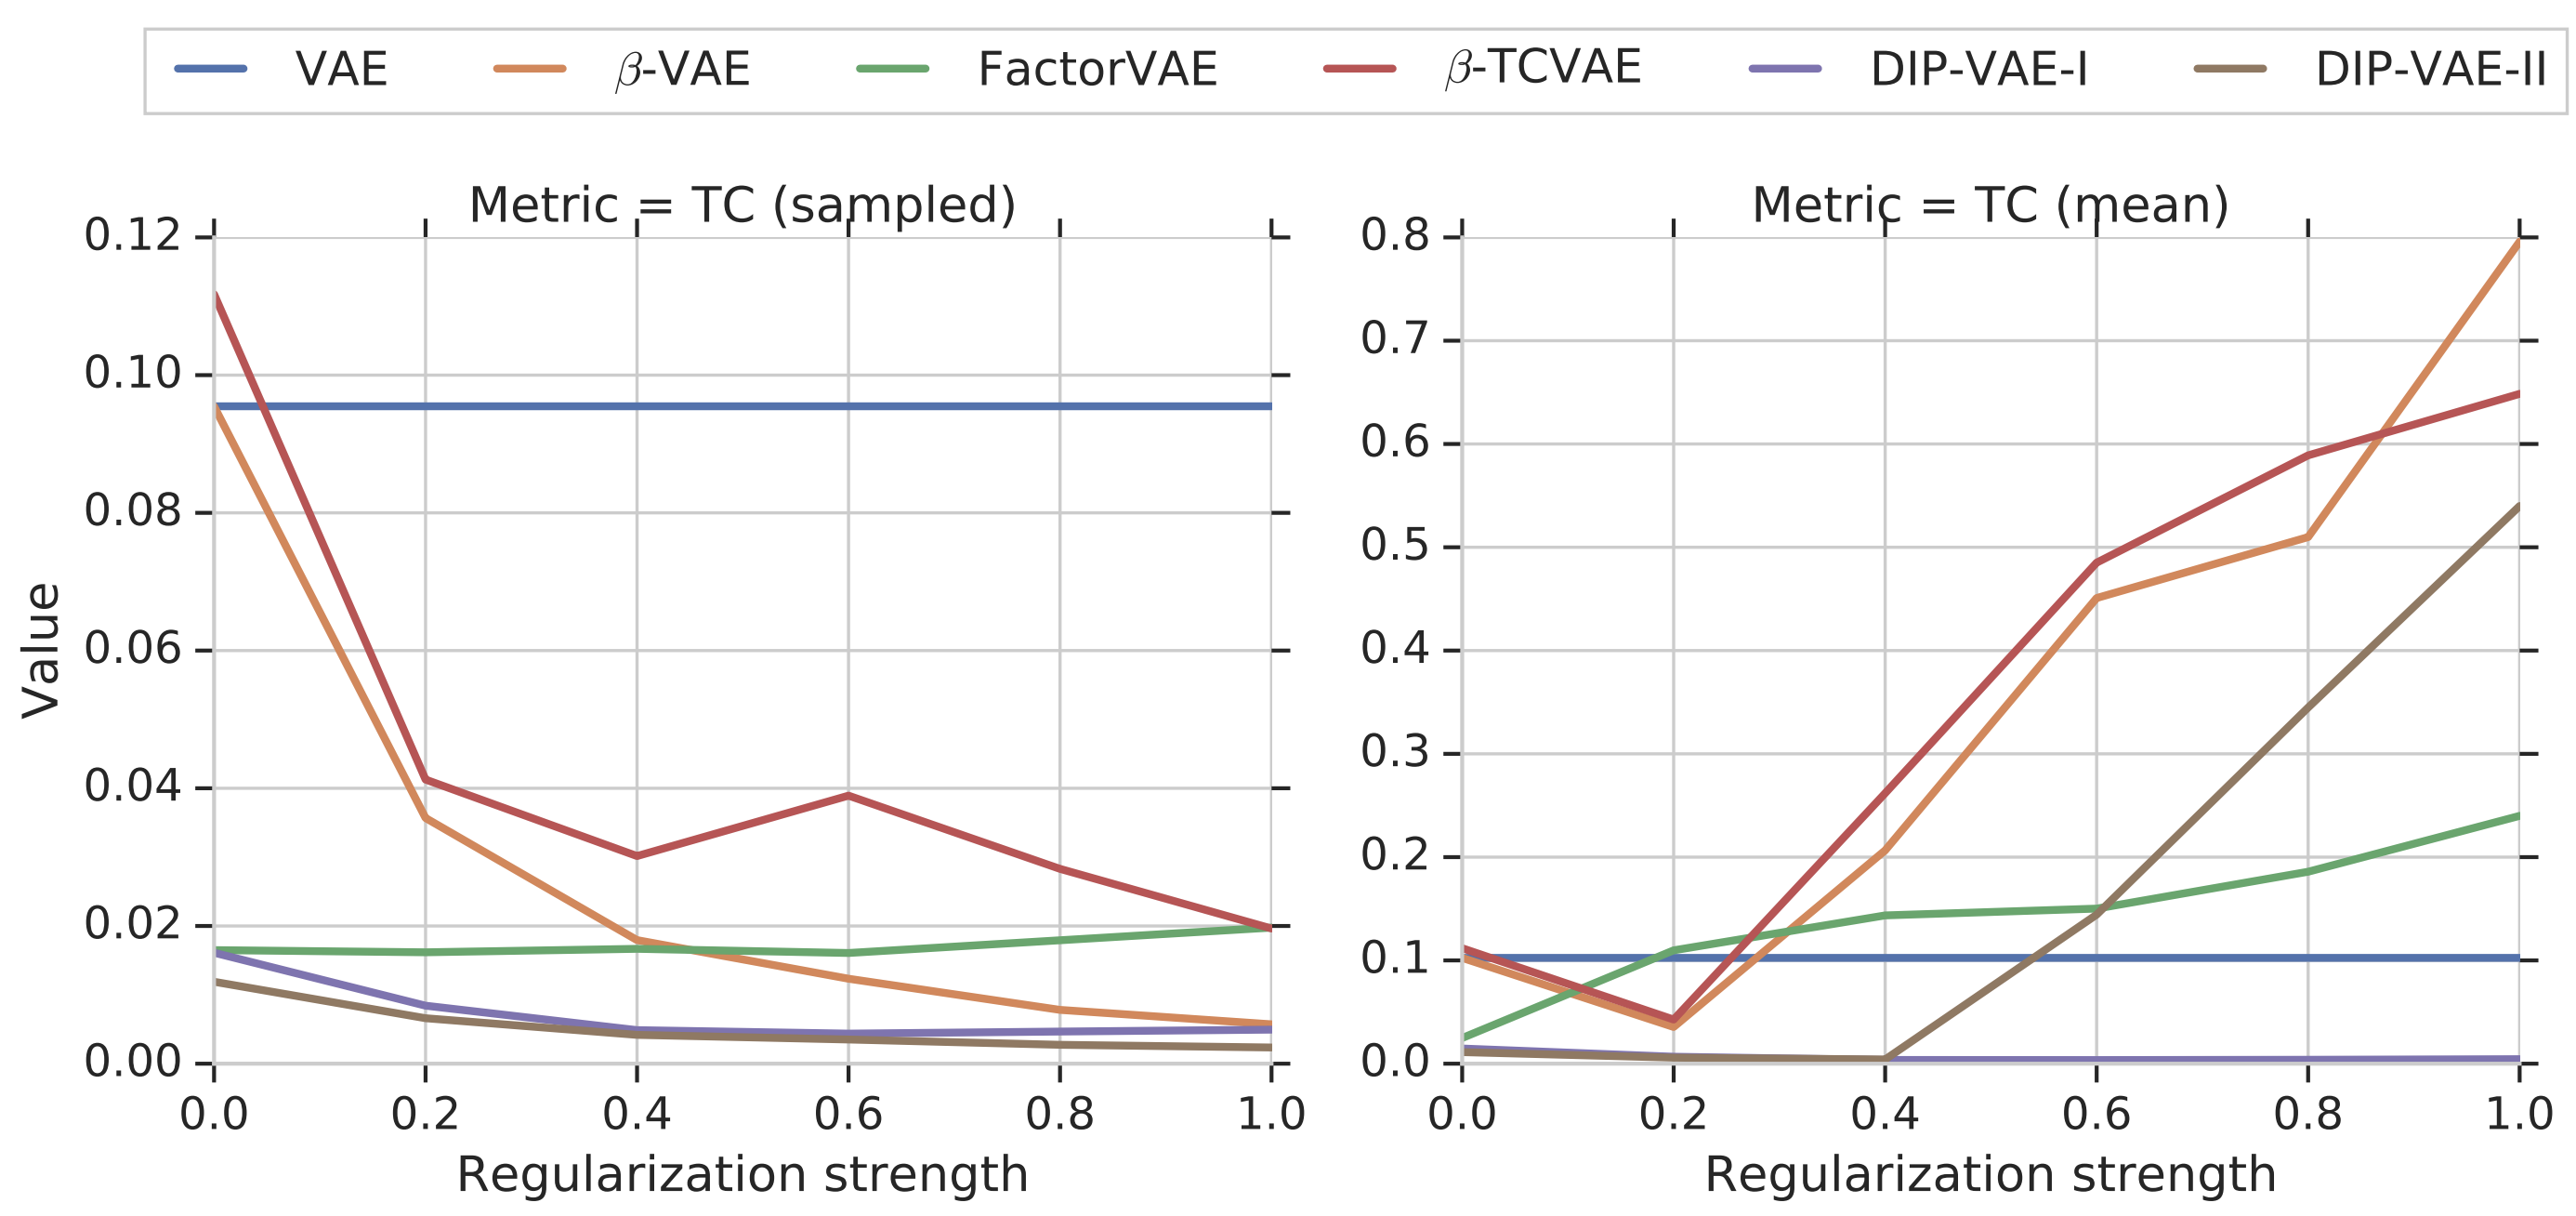
\includegraphics[width=0.95\linewidth]{figs/challenge_dis_1}
\end{figure}

\myfootnotewithlink{https://arxiv.org/abs/1811.12359}{Locatello F. et al. Challenging Common Assumptions in the Unsupervised Learning of Disentangled Representations, 2018}
\end{frame}
%=======
\begin{frame}{Challenging Disentanglement Assumptions}
\begin{block}{Importance of different models and hyperparameters for disentanglement}
	\begin{figure}
		\centering
		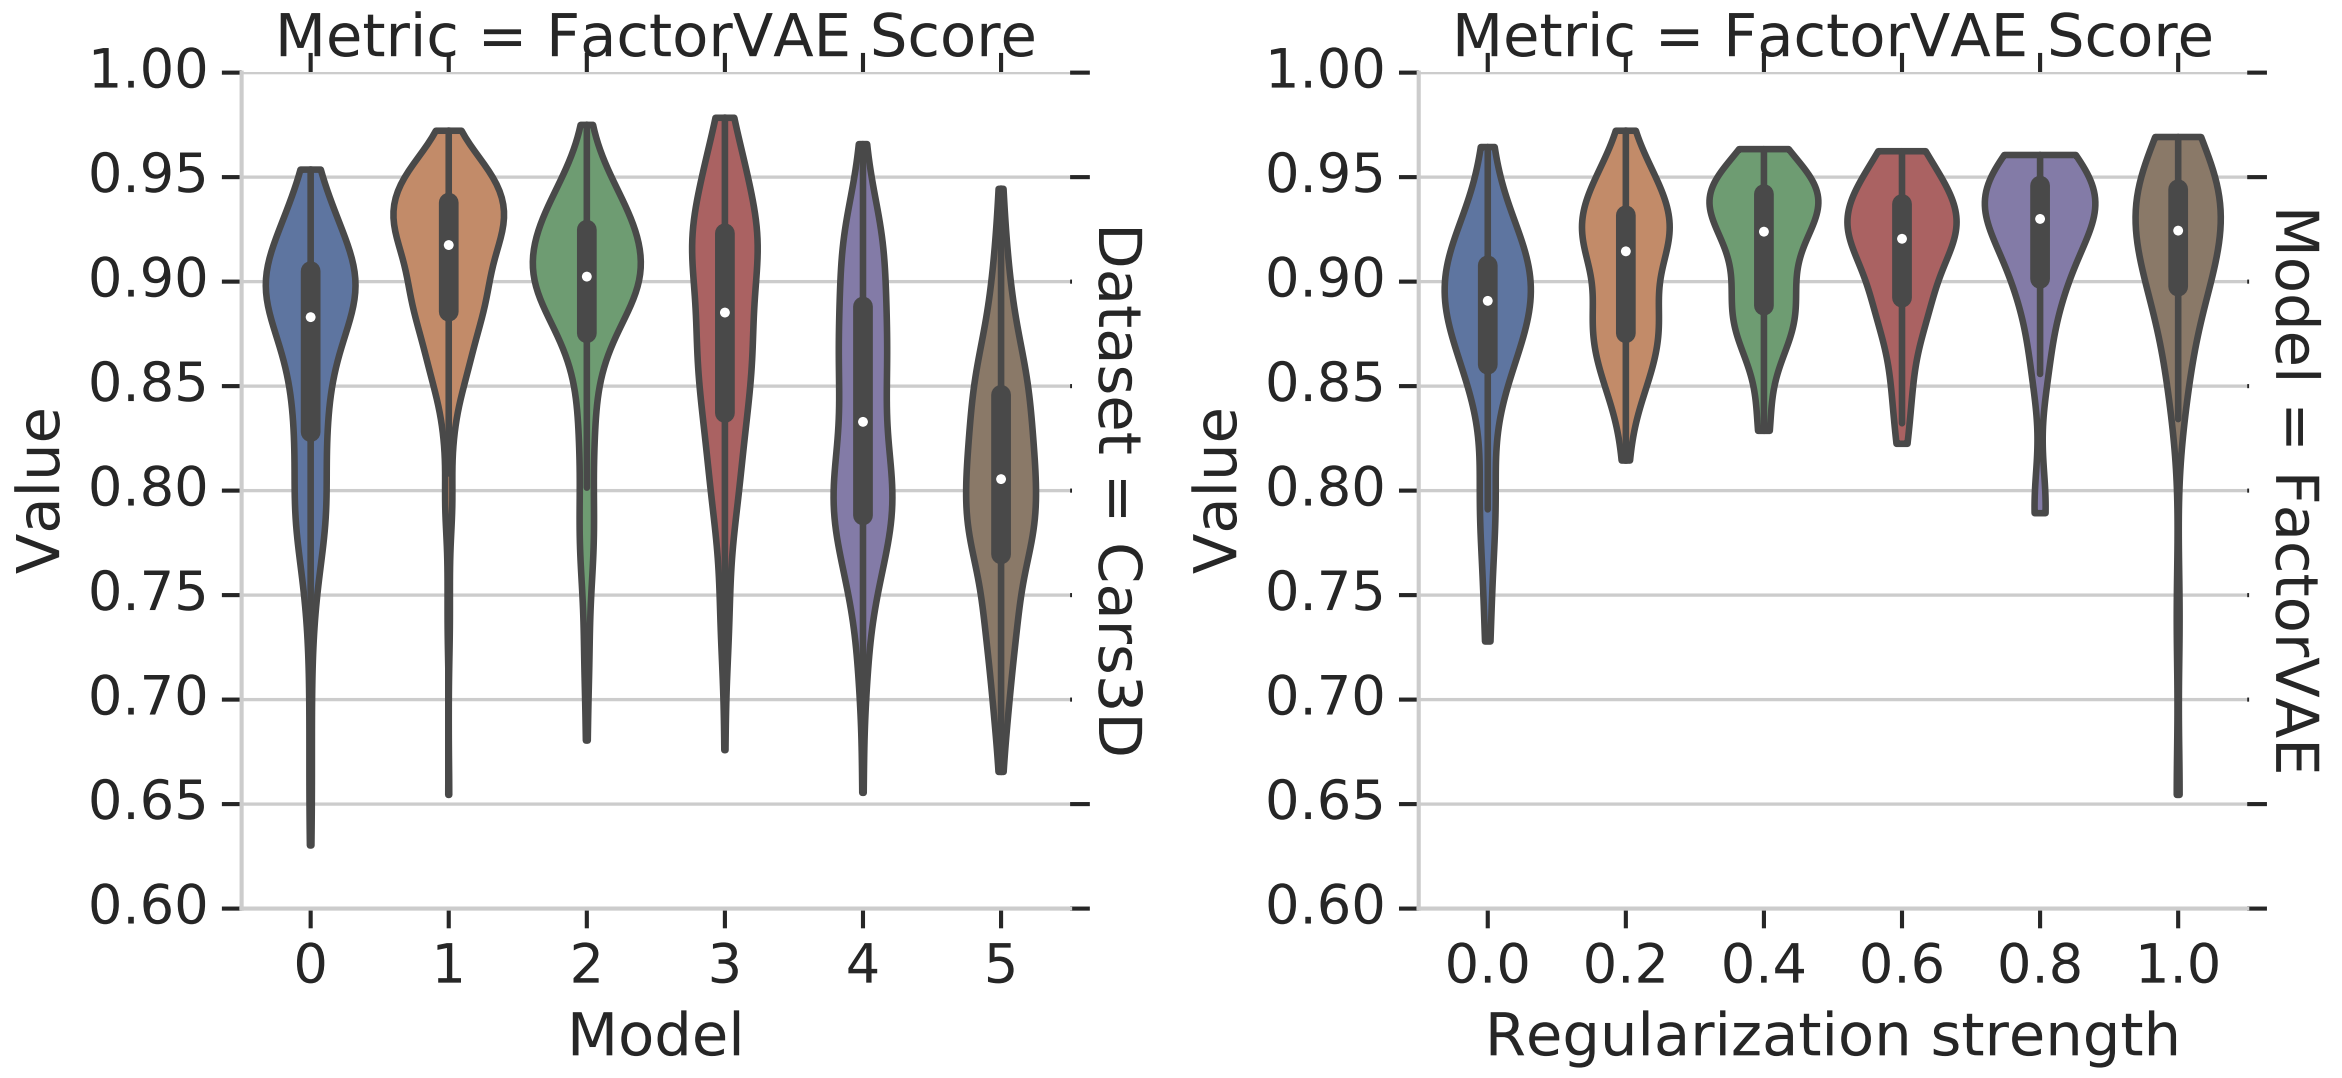
\includegraphics[width=\linewidth]{figs/challenge_dis_2}
	\end{figure}
\end{block}

\myfootnotewithlink{https://arxiv.org/abs/1811.12359}{Locatello F. et al. Challenging Common Assumptions in the Unsupervised Learning of Disentangled Representations, 2018}
\end{frame}
%=======
\begin{frame}{Challenging Disentanglement Assumptions}
\begin{block}{Agreement of different disentanglement metrics}
	\begin{figure}
		\centering
		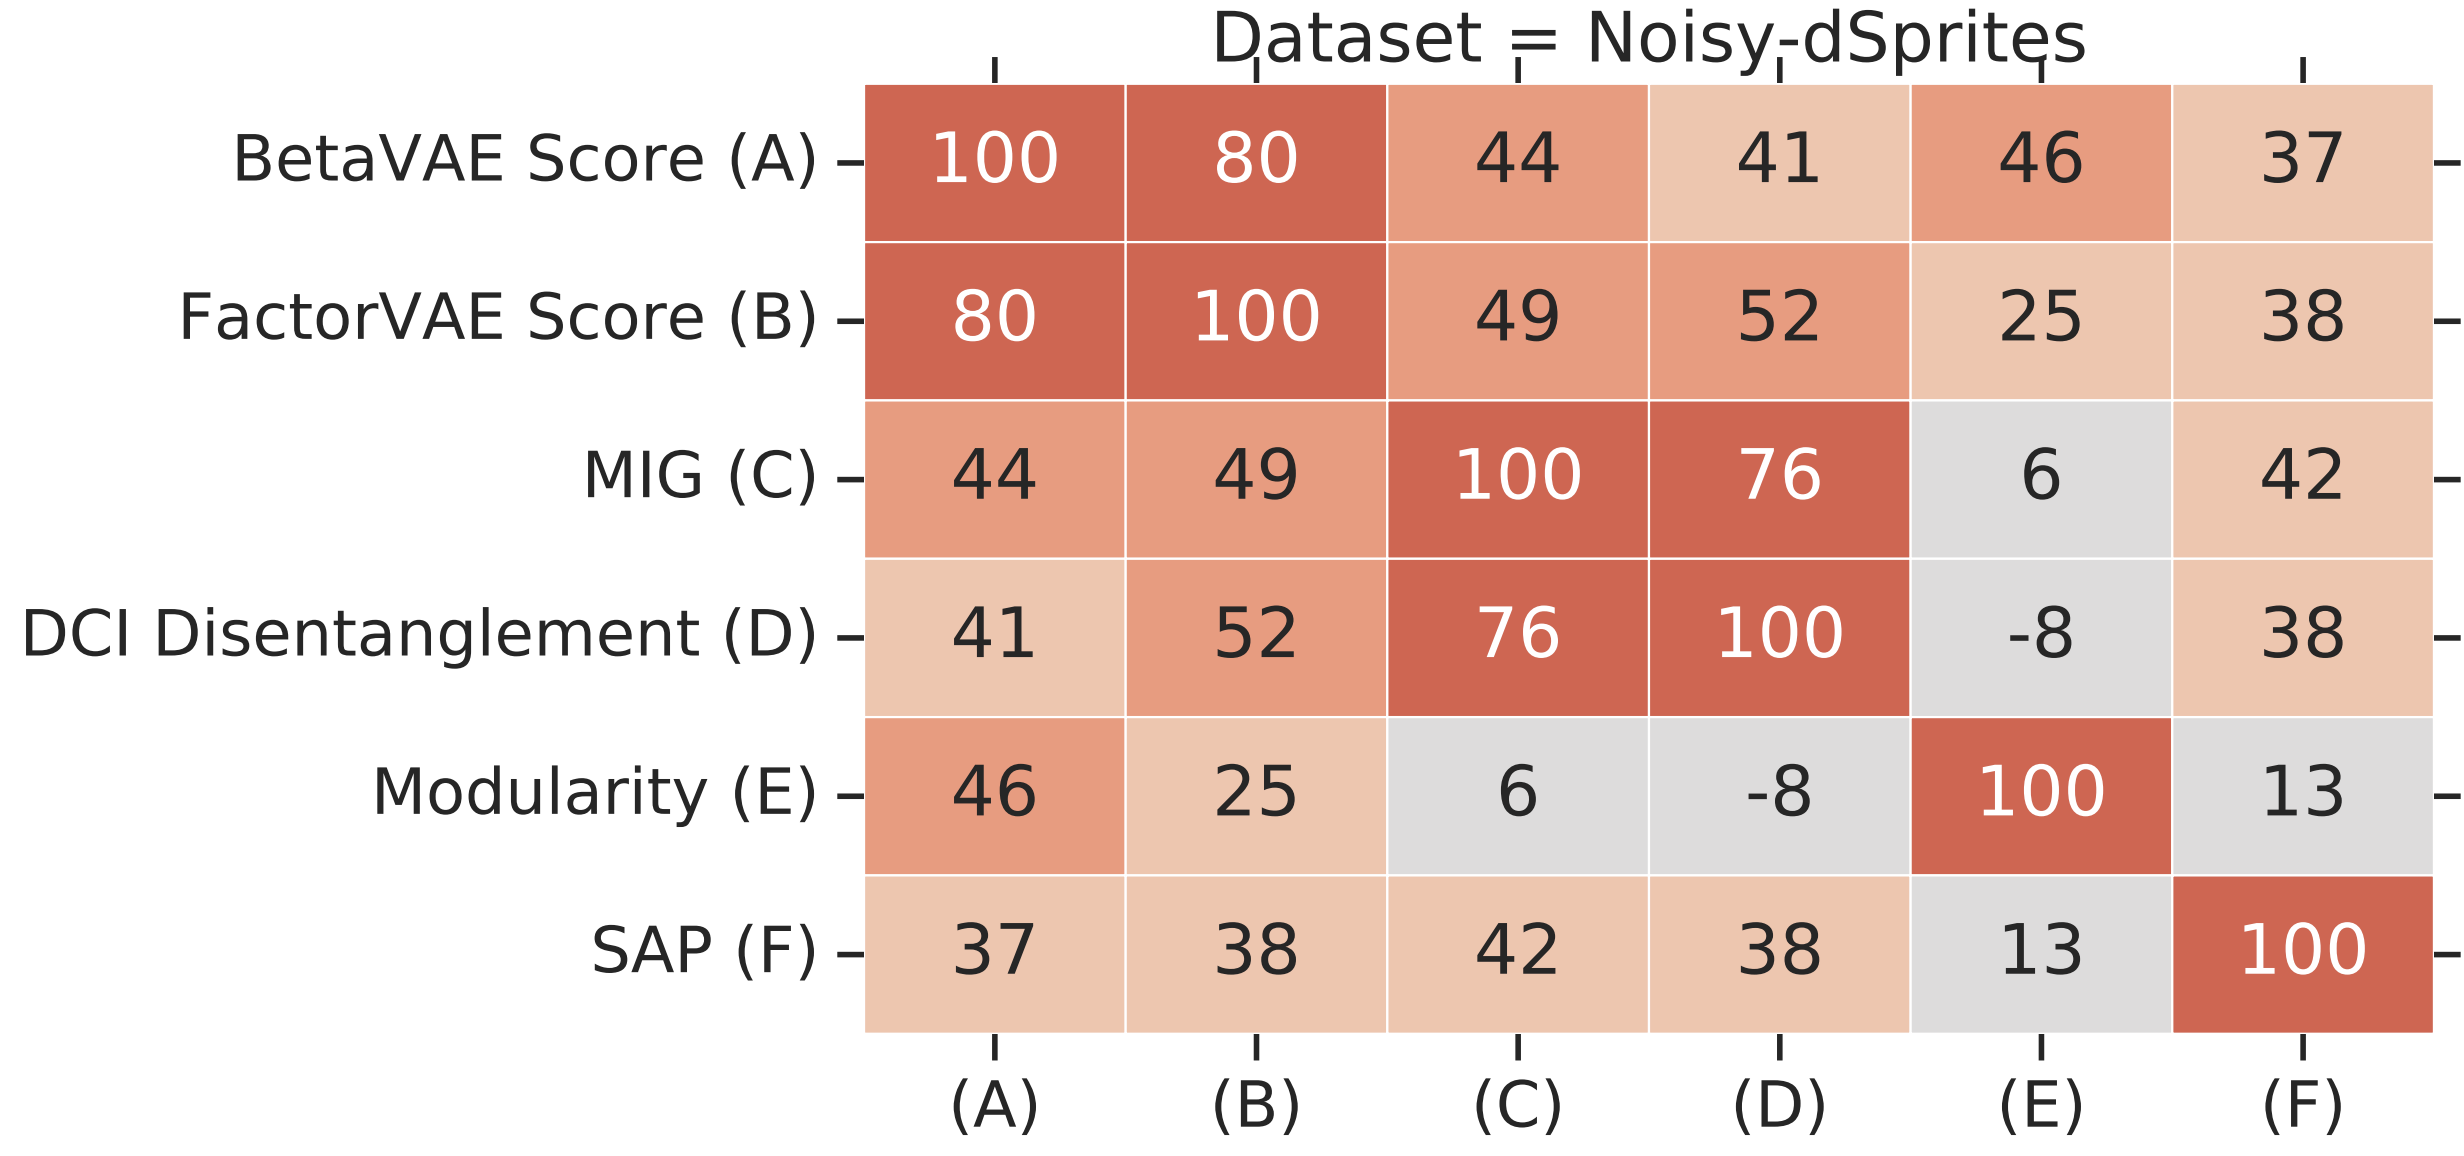
\includegraphics[width=0.9\linewidth]{figs/challenge_dis_3}
	\end{figure}
	\vspace{0.5cm}
\end{block}

\myfootnotewithlink{https://arxiv.org/abs/1811.12359}{Locatello F. et al. Challenging Common Assumptions in the Unsupervised Learning of Disentangled Representations, 2018}
\end{frame}
%=======
\begin{frame}{Generative models zoo}
	\begin{figure}
		\centering
		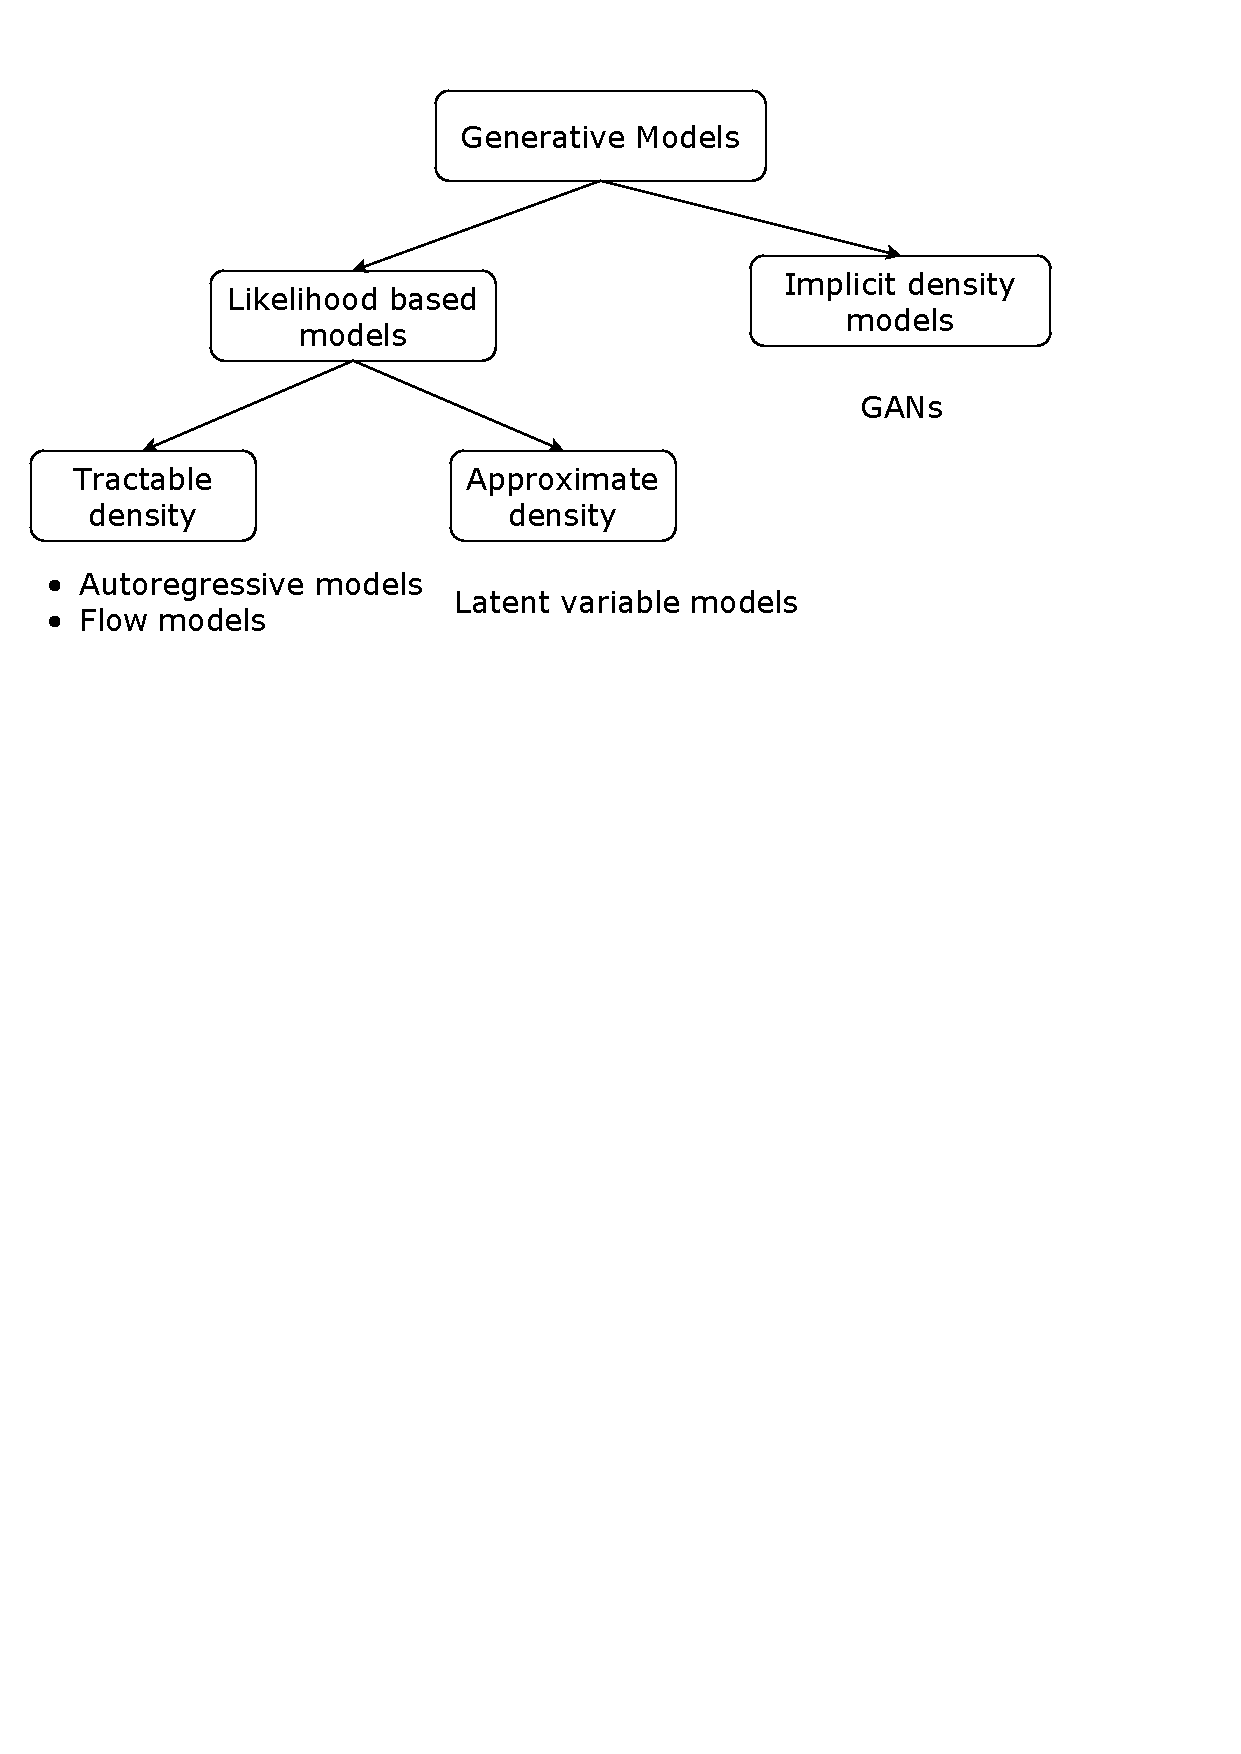
\includegraphics[width=1.0\linewidth]{figs/generative_models_zoo.pdf}
	\end{figure}
\end{frame}
%=======
\begin{frame}{Likelihood based models}
	Is likelihood a good measure of model quality?
	\begin{minipage}[t]{0.48\columnwidth}
		\begin{block}{Poor likelihood \\ Great samples}
			\vspace{-0.3cm}
			\[
				p_1(\bx) = \frac{1}{n} \sum_{i=1}^n \cN(\bx | \bx_i, \epsilon \bI)
			\]
			For small $\epsilon$ this model will generate samples with great quality, but likelihood will be very poor.
		\end{block}
	\end{minipage}%
	\begin{minipage}[t]{0.52\columnwidth}
		\begin{block}{Great likelihood \\ Poor samples}
			\vspace{-0.3cm}
			\[
				p_2(\bx) = 0.01p(\bx) + 0.99p_{\text{noise}}(\bx)
			\]
			\begin{multline*}
				\log \left[ 0.01p(\bx) + 0.99p_{\text{noise}}(\bx) \right] \geq  \\ \geq \log \left[ 0.01p(\bx) \right]  = \log p(\bx) - \log 100
			\end{multline*}
		Noisy irrelevant samples, but for high dimensions $\log p(\bx)$ becames larger.
		\end{block}
	\end{minipage}
	\myfootnotewithlink{https://arxiv.org/abs/1511.01844}{Theis L., Oord A., Bethge M. A note on the evaluation of generative models, 2015}
\end{frame}
%=======
\begin{frame}{Likelihood-free learning}
	\begin{itemize}
		\item Likelihood is not a perfect measure quality measure for generative model.
		\item Likelihood could be intractable.
	\end{itemize}
	\begin{block}{Where did we start}
	 We would like to approximate true data distribution $\pi(\bx)$.
		Instead of searching true $\pi(\bx)$ over all probability distributions, learn function approximation $p(\bx | \btheta) \approx \pi(\bx)$.
	\end{block}
	Imagine we have two sets of samples 
	\begin{itemize}
		\item $\cS_1 = \{\bx_i\}_{i=1}^{n_1} \sim \pi(\bx)$ -- real samples;
		\item $\cS_2 = \{\bx_i\}_{i=1}^{n_2} \sim p(\bx | \btheta)$ -- generated (or fake) samples.
	\end{itemize}
	\begin{block}{Two sample test}
		\vspace{-0.3cm}
		\[
			H_0: \pi(\bx) = p(\bx | \btheta), \quad H_1: \pi(\bx) \neq p(\bx | \btheta)
		\]
	\end{block}
	Define test statistic $T(\cS_1, \cS_2)$. The test statistic is likelihood free.
	If $T(\cS_1, \cS_2) < \alpha$, then accept $H_0$, else reject it.
\end{frame}
%=======
\begin{frame}{Likelihood-free learning}
	\begin{block}{Two sample test}
		\vspace{-0.3cm}
		\[
			H_0: \pi(\bx) = p(\bx | \btheta), \quad H_1: \pi(\bx) \neq p(\bx | \btheta)
		\]
		\vspace{-0.6cm}
	\end{block}
	\begin{block}{Desired behaviour}
		\begin{itemize}
			\item $p(\bx | \btheta)$ minimizes the value of test statistic~$T(\cS_1, \cS_2)$.
			\item It is hard to find an appropriate test statistic in high dimensions. $T(\cS_1, \cS_2)$ could be learnable.
		\end{itemize}
	\end{block}
	\begin{block}{GAN objective}
		\vspace{-0.5cm}
		\[
			\min_{G} \max_D V(G, D) = \min_{G} \max_D \left[ \bbE_{\pi(\bx)} \log D(\bx) + \bbE_{p(\bz)} \log (1 - D(G(\bz))) \right]
		\]
		\vspace{-0.4cm}
	\end{block}
	\begin{itemize}
		\item \textbf{Generator:} generative model $\bx = G(\bz)$, which makes generated sample more realistic.
		\item \textbf{Discriminator:} a classifier $D(\bx) \in [0, 1]$, which distinguishes real samples from generated samples.
	\end{itemize}
	 \myfootnotewithlink{https://arxiv.org/abs/1406.2661}{Goodfellow I. J. et al. Generative Adversarial Networks, 2014}
\end{frame}
%=======
\begin{frame}{Vanilla GAN optimality}
	\begin{block}{Theorem}
	The minimax game 
		\vspace{-0.1cm}
		\[
			\min_{G} \max_D V(G, D) = \min_{G} \max_D \left[ \bbE_{\pi(\bx)} \log D(\bx) + \bbE_{p(\bz)} \log (1 - D(G(\bz))) \right]
		\]
	has the global optimum $\pi(\bx) = p(\bx | \btheta)$, in this case $D(\bx) = 0.5$.
	\end{block}
	\begin{block}{Proof (fixed $G$)}
		\vspace{-0.5cm}
		\begin{align*}
			V(G, D) &= \bbE_{\pi(\bx)} \log D(\bx) + \bbE_{p(\bx | \btheta)} \log (1 - D(\bx)) \\
			&= \int \underbrace{\left[ \pi(\bx) \log D(\bx) + p(\bx | \btheta)\log (1 - D(\bx) \right]}_{y(D)} d \bx
		\end{align*}
		\vspace{-0.2cm}
		\[
			\frac{d y(D)}{d D} = \frac{\pi(\bx)}{D(\bx)} - \frac{p(\bx | \btheta)}{1 - D(\bx)} = 0 \quad \Rightarrow \quad D^*(\bx) = \frac{\pi(\bx)}{\pi(\bx) + p(\bx | \btheta)}
		\]
	\end{block}
	\myfootnotewithlink{https://arxiv.org/abs/1406.2661}{Goodfellow I. J. et al. Generative Adversarial Networks, 2014}
\end{frame}
%=======
\begin{frame}{Vanilla GAN optimality}
	\begin{block}{Proof confitnued (fixed $D$)}
		\vspace{-0.5cm}
		\begin{multline*}
			V(G, D^*) = \bbE_{\pi(\bx)} \log \frac{\pi(\bx)}{\pi(\bx) + p(\bx | \btheta)} + \bbE_{p(\bx | \btheta)} \log \frac{p(\bx | \btheta)}{\pi(\bx) + p(\bx | \btheta)} \\
		 = KL \left(\pi(\bx) || \frac{\pi(\bx) + p(\bx | \btheta)}{2}\right) + KL \left(p(\bx | \btheta) || \frac{\pi(\bx) + p(\bx | \btheta)}{2}\right) - 2\log 2 \\
		 = 2JSD(\pi(\bx) || p(\bx | \btheta)) - 2\log 2.
		\end{multline*}
	\end{block}
	\vspace{-0.3cm}
	\begin{block}{Jensen-Shannon divergence (symmetric KL divergence)}
		\vspace{-0.2cm}
		\footnotesize
		\[
			JSD(\pi(\bx) || p(\bx | \btheta)) = \frac{1}{2} \left[KL \left(\pi(\bx) || \frac{\pi(\bx) + p(\bx | \btheta)}{2}\right) + KL \left(p(\bx | \btheta) || \frac{\pi(\bx) + p(\bx | \btheta)}{2}\right) \right]
		\]
	\end{block}
	Could be used as a distance measure!
	\[
		V(G^*, D^*) = -2\log 2, \quad \pi(\bx) = p(\bx | \btheta).
	\]
	
	 \myfootnotewithlink{https://arxiv.org/abs/1406.2661}{Goodfellow I. J. et al. Generative Adversarial Networks, 2014}
\end{frame}
%=======
\begin{frame}{Vanilla GAN optimality}
	\begin{block}{Theorem}
		The minimax game 
		\vspace{-0.1cm}
		\[
			\min_{G} \max_D  V(G, D) = \min_{G} \max_D \left[ \bbE_{\pi(\bx)} \log D(\bx) + \bbE_{p(\bz)} \log (1 - D(G(\bz))) \right]
		\]
		has the global optimum $\pi(\bx) = p(\bx | \btheta)$, in this case $D(\bx) = 0.5$.
	\end{block}
	\vspace{-0.2cm}
	\begin{block}{Proof}
	for fixed $G$:
	\[
		D^*(\bx) = \frac{\pi(\bx)}{\pi(\bx) + p(\bx | \btheta)}
	\]
	\vspace{-0.5cm} \\
	for fixed $D$:
	\[
		\min_{G} V(G, D^*) = \min_{G} \left[ JSD(\pi || p) - \log 4 \right] = -\log 4, \quad \pi(\bx) = p(\bx | \btheta).
	\]
	\vspace{-0.6cm}
	\end{block}
	If the generator could be any function and the discriminator is optimal at every step, then the generator is guaranteed to converge to the data distribution.
	 \myfootnotewithlink{https://arxiv.org/abs/1406.2661}{Goodfellow I. J. et al. Generative Adversarial Networks, 2014}
\end{frame}
%=======
\begin{frame}{Vanilla GAN}
	\begin{block}{Objective}
		\vspace{-0.4cm}
		\[
		\min_{G} \max_D V(G, D) = \min_{G} \max_D \left[ \bbE_{\pi(\bx)} \log D(\bx) + \bbE_{p(\bz)} \log (1 - D(G(\bz))) \right]
		\]
		\vspace{-0.4cm}
	\end{block}

	\begin{figure}
		\centering
		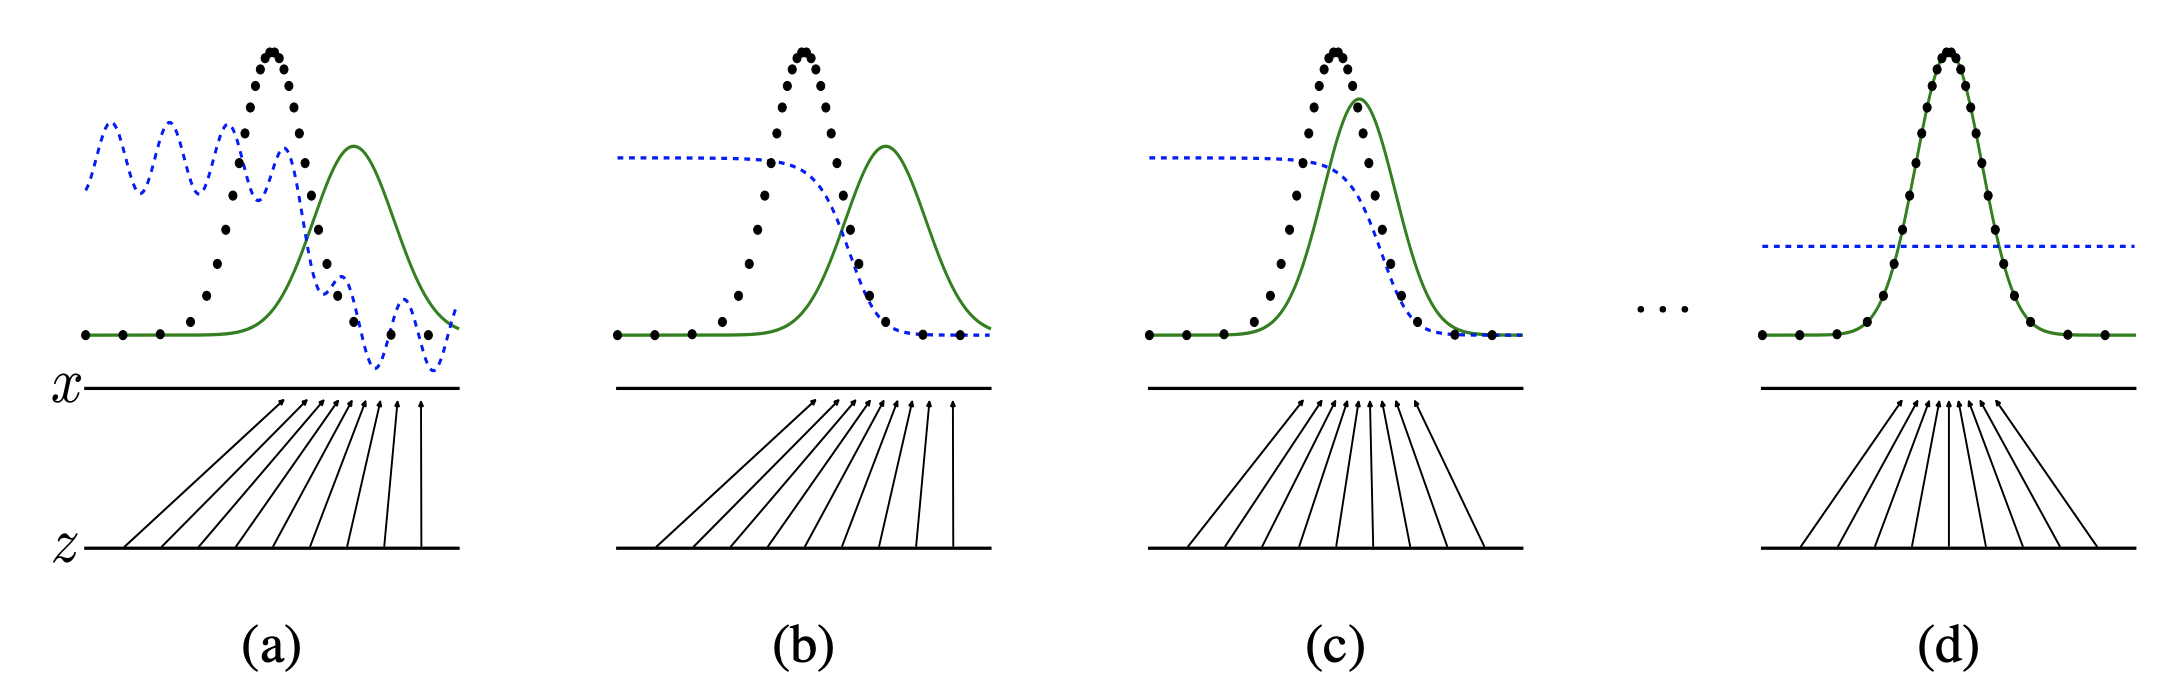
\includegraphics[width=1.0\linewidth]{figs/gan_1}
	\end{figure}
	\begin{itemize}
		\item Generator updates are made in parameter space.
		\item Discriminator is not optimal at every step.
		\item Generator and discriminator loss keeps oscillating during GAN training.
	\end{itemize}

	 \myfootnotewithlink{https://arxiv.org/abs/1406.2661}{Goodfellow I. J. et al. Generative Adversarial Networks, 2014}
\end{frame}
%=======
\begin{frame}{Vanishing gradients}
	\begin{block}{Objective}
		\vspace{-0.4cm}
		\[
		\min_{G} \max_D V(G, D) = \min_{G} \max_D \left[ \bbE_{\pi(\bx)} \log D(\bx) + \bbE_{p(\bz)} \log (1 - D(G(\bz))) \right]
		\]
		\vspace{-0.4cm}
	\end{block}
	Early in learning, $G$ is poor, $D$ can reject samples with high confidence. In this case, $\log (1 - D(G(\bz)))$ saturates.
	\begin{minipage}[t]{0.5\columnwidth}
		\begin{figure}
			\centering
			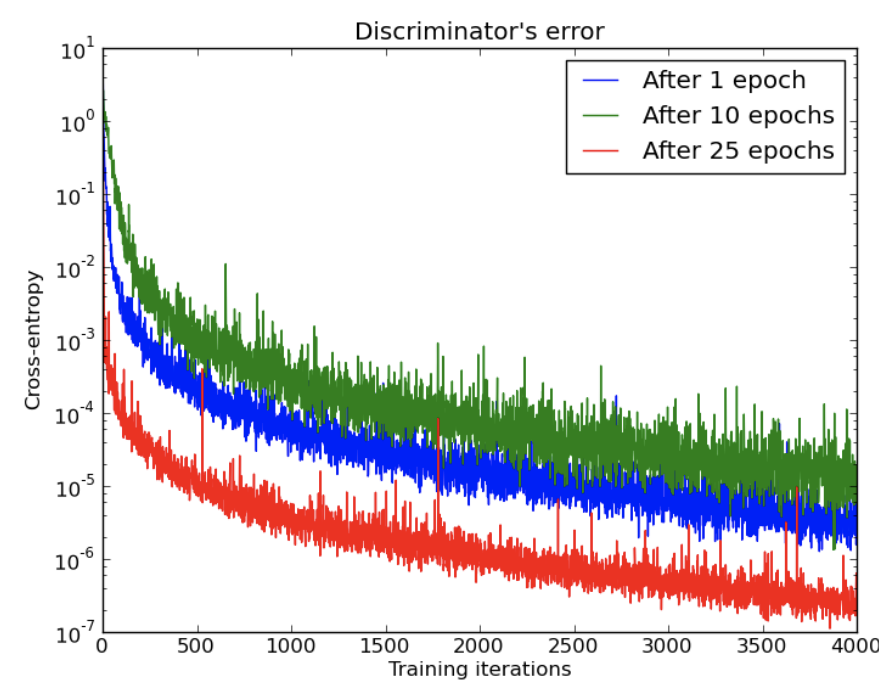
\includegraphics[width=0.9\linewidth]{figs/vanishing_gradients_1}
		\end{figure}
	\end{minipage}%
	\begin{minipage}[t]{0.5\columnwidth}
		\begin{figure}
			\centering
			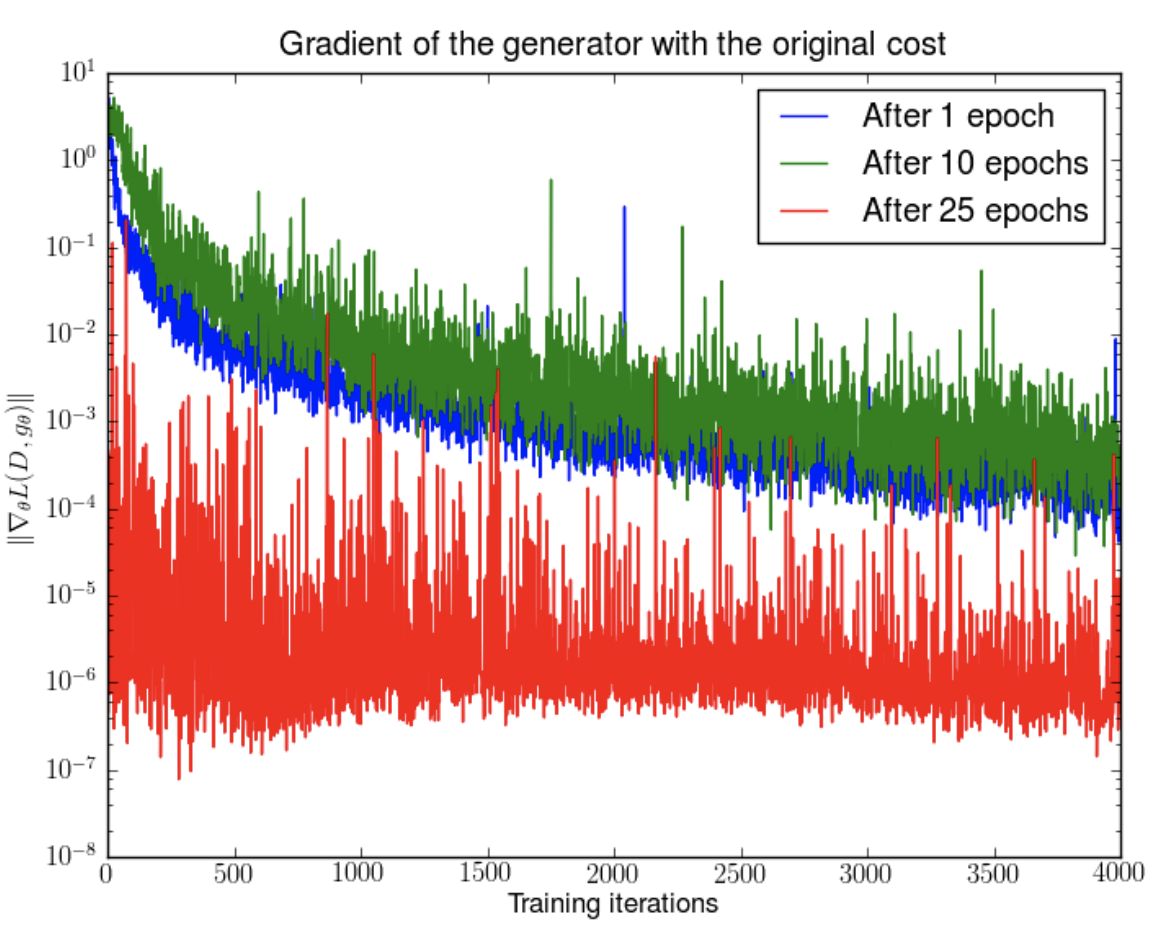
\includegraphics[width=0.9\linewidth]{figs/vanishing_gradients_2}
		\end{figure}
	\end{minipage}
	\myfootnotewithlink{https://arxiv.org/abs/1701.04862}{Arjovsky M., Bottou L. Towards Principled Methods for Training Generative Adversarial Networks, 2017}
\end{frame}
%=======
\begin{frame}{Vanishing gradients}
	\begin{block}{Objective}
		\vspace{-0.4cm}
		\[
		\min_{G} \max_D V(G, D) = \min_{G} \max_D \left[ \bbE_{\pi(\bx)} \log D(\bx) + \bbE_{p(\bz)} \log (1 - D(G(\bz))) \right]
		\]
		\vspace{-0.4cm}
	\end{block}
	\begin{minipage}[t]{0.45\columnwidth}
		\begin{block}{Non-saturating GAN}
		\begin{itemize}
			\item Maximize $\log D(G(z))$ instead of $\log (1 - D(G(\bz)))$. \\
			\item Gradients are getting much stronger, but the training is instable (with increasing mean and variance).
		\end{itemize}
		\end{block}
	\end{minipage}%
	\begin{minipage}[t]{0.55\columnwidth}
		\begin{figure}
			\centering
			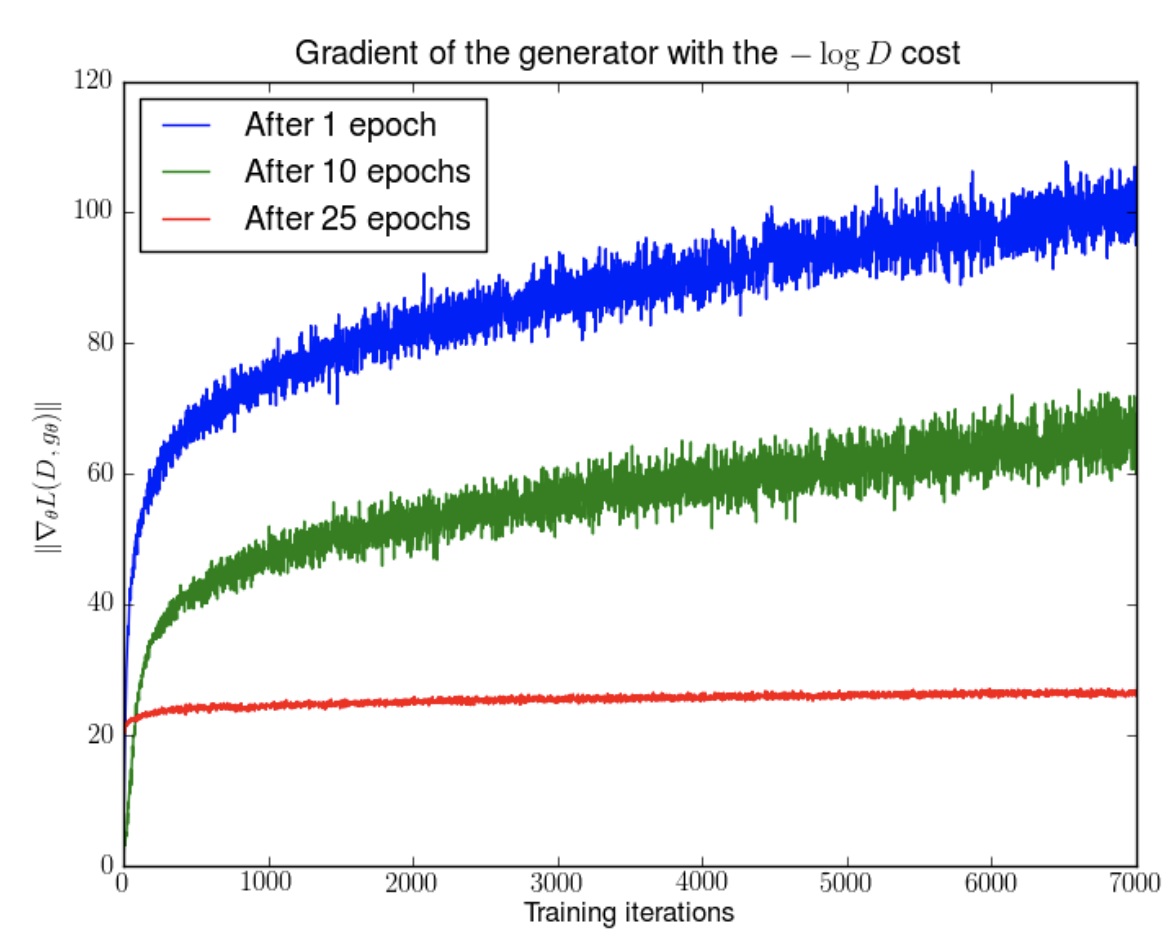
\includegraphics[width=1.0\linewidth]{figs/vanishing_gradients_3}
		\end{figure}
	\end{minipage}
	\myfootnotewithlink{https://arxiv.org/abs/1701.04862}{Arjovsky M., Bottou L. Towards Principled Methods for Training Generative Adversarial Networks, 2017}
\end{frame}
%=======
\begin{frame}{Mode collapse}
	The phenomena where the generator of a GAN collapses to one or few distribution modes.
	\begin{figure}
		\centering
		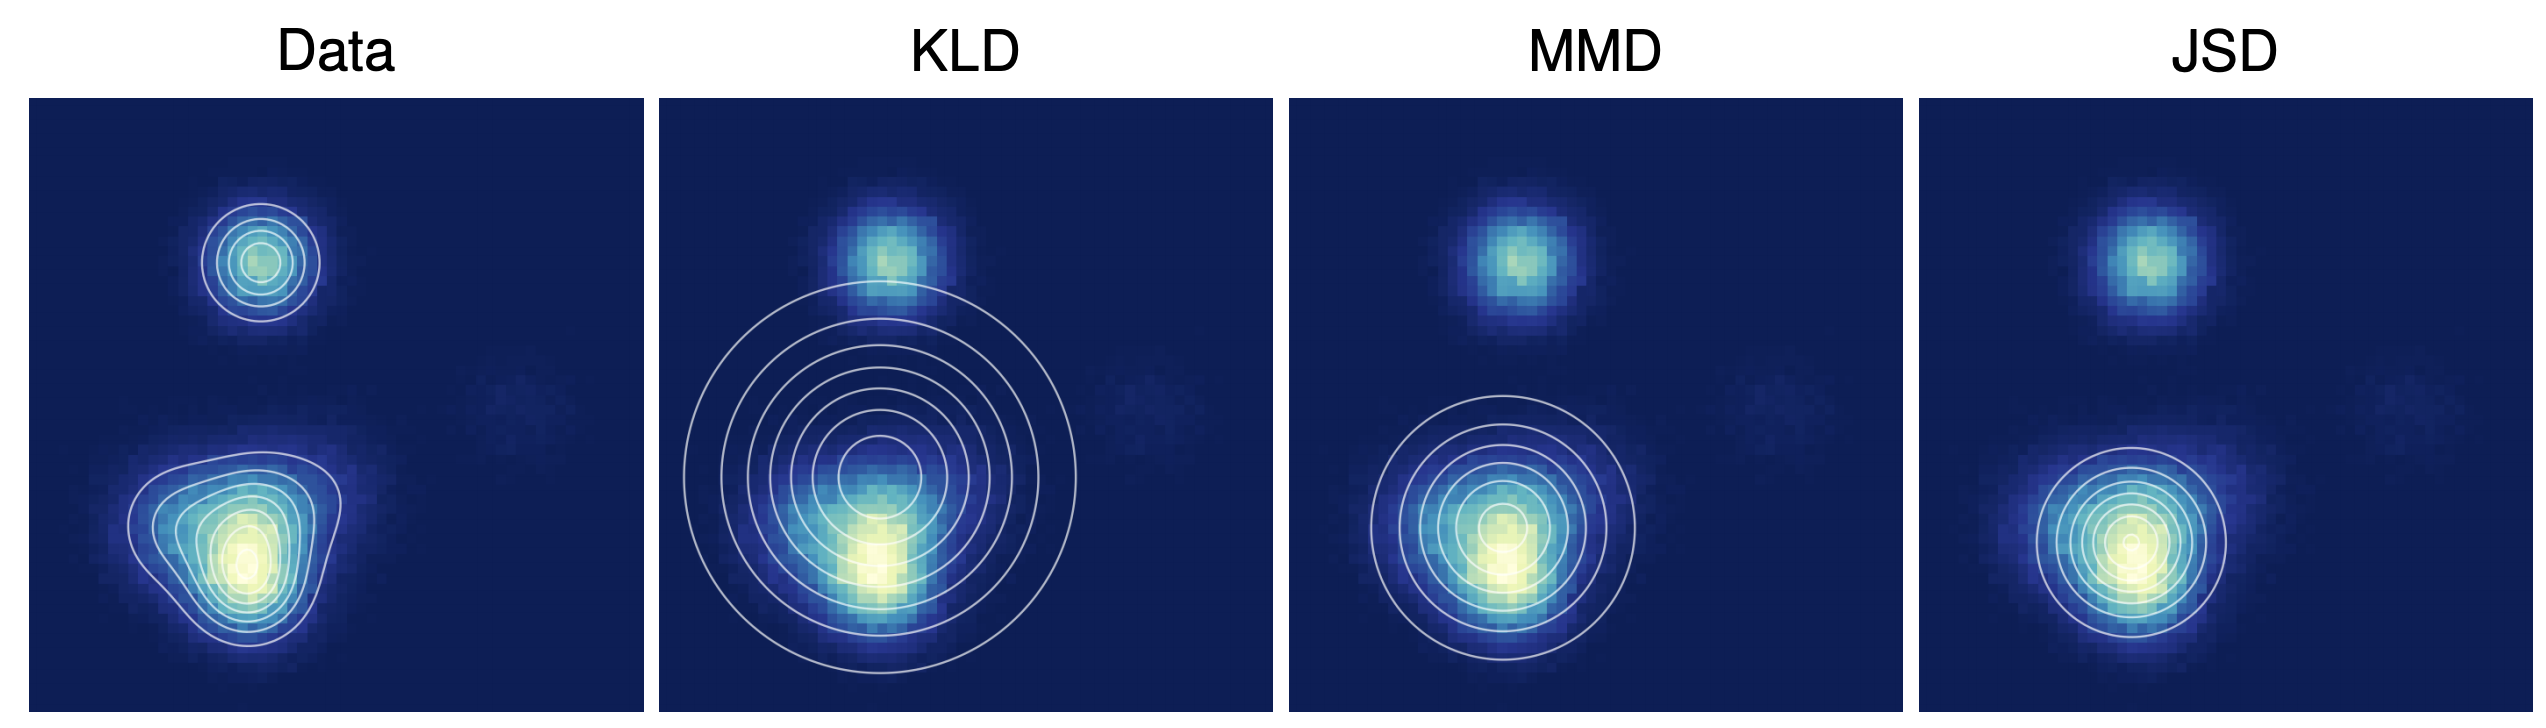
\includegraphics[width=0.9\linewidth]{figs/mode_collapse_1}
	\end{figure}
	\begin{figure}
		\centering
		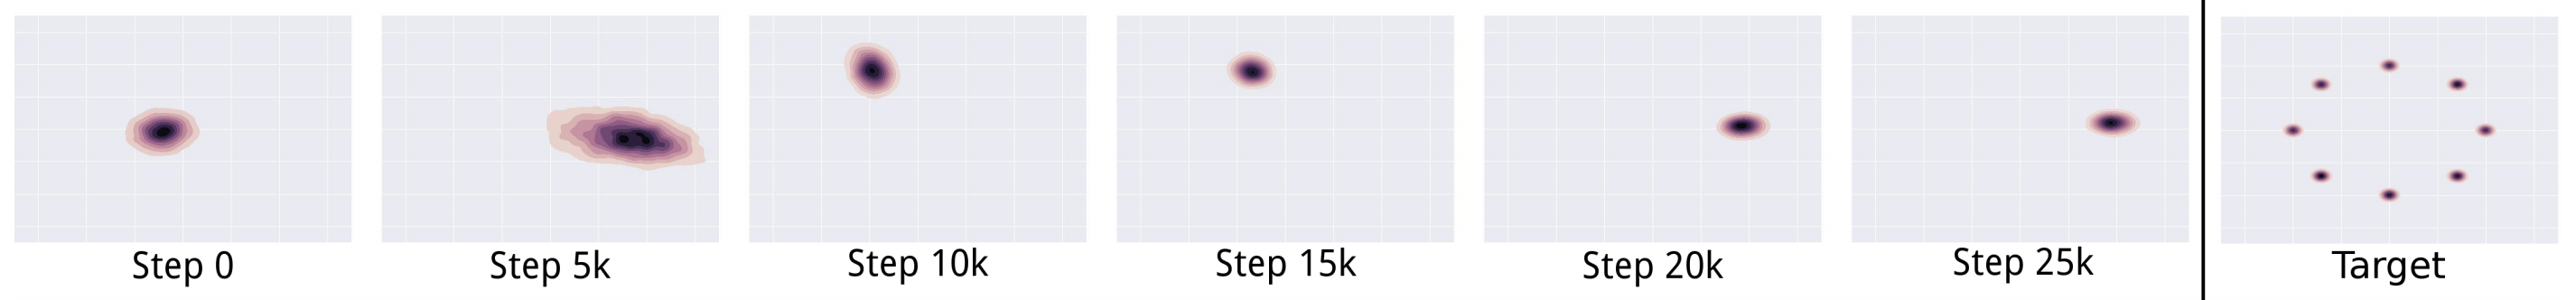
\includegraphics[width=1.0\linewidth]{figs/mode_collapse_3}
	\end{figure}
	Alternate architectures, adding regularization terms, injecting small noise
	perturbations and other millions bags and tricks are used to avoid the mode collapse.
	
	\myfootnote{\href{https://arxiv.org/abs/1406.2661}{Goodfellow I. J. et al. Generative Adversarial Networks, 2014} \\
	\href{https://arxiv.org/abs/1611.02163}{Metz L. et al. Unrolled Generative Adversarial Networks, 2016}}
\end{frame}
%=======
\begin{frame}{Jensen-Shannon vs Kullback-Leibler }
	\begin{block}{Mode covering vs mode seeking}
		\vspace{-0.2cm}
		\[
			KL(\pi || p) = \int \pi(\bx) \log \frac{\pi(\bx)}{p(\bx)}d\bx, \quad KL(p || \pi) = \int p(\bx) \log \frac{p(\bx)}{\pi(\bx)}d\bx
		\]
		\[
		JSD(\pi || p) = \frac{1}{2} \left[KL \left(\pi(x) || \frac{\pi(\bx) + p(\bx)}{2}\right) + KL \left(p(x) || \frac{\pi(\bx) + p(\bx)}{2}\right) \right]
		\]
		\vspace{-0.4cm}
		\begin{figure}
			\centering
			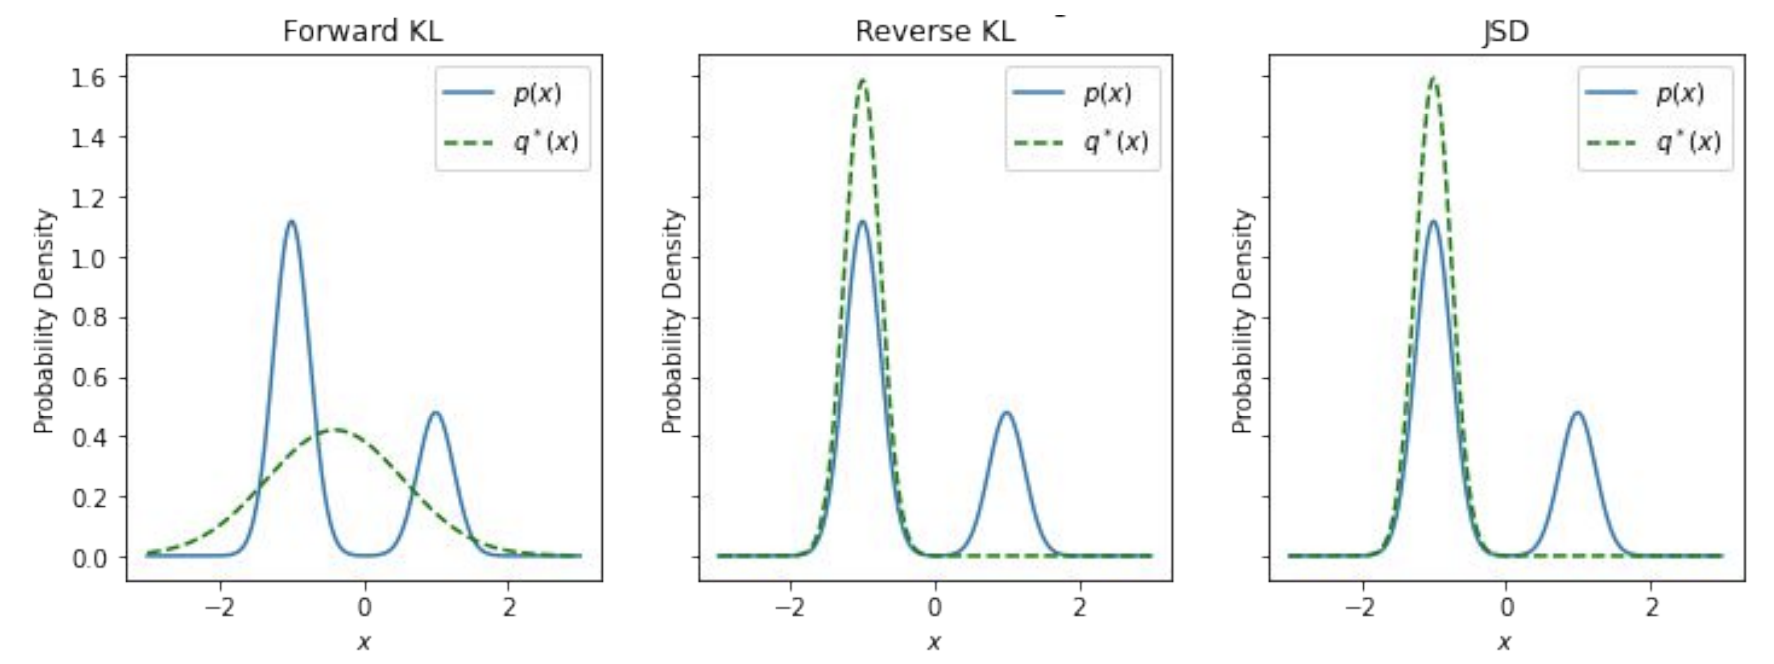
\includegraphics[width=0.7\linewidth]{figs/mode_collapse_2}
		\end{figure}
	\vspace{-0.3cm}
	\end{block}
	\myfootnotewithlink{https://sites.google.com/view/berkeley-cs294-158-sp20/home}{image credit: https://sites.google.com/view/berkeley-cs294-158-sp20/home}
\end{frame}
%=======
\begin{frame}{Vanilla GAN results}
	\begin{figure}
		\centering
		\includegraphics[width=0.95\linewidth]{figs/Vanila_gan_results}
	\end{figure}
	\myfootnotewithlink{https://arxiv.org/abs/1406.2661}{Goodfellow I. J. et al. Generative Adversarial Networks, 2014}
\end{frame}
%=======
\begin{frame}{Deep Convolutional GAN}
	\begin{figure}
		\centering
		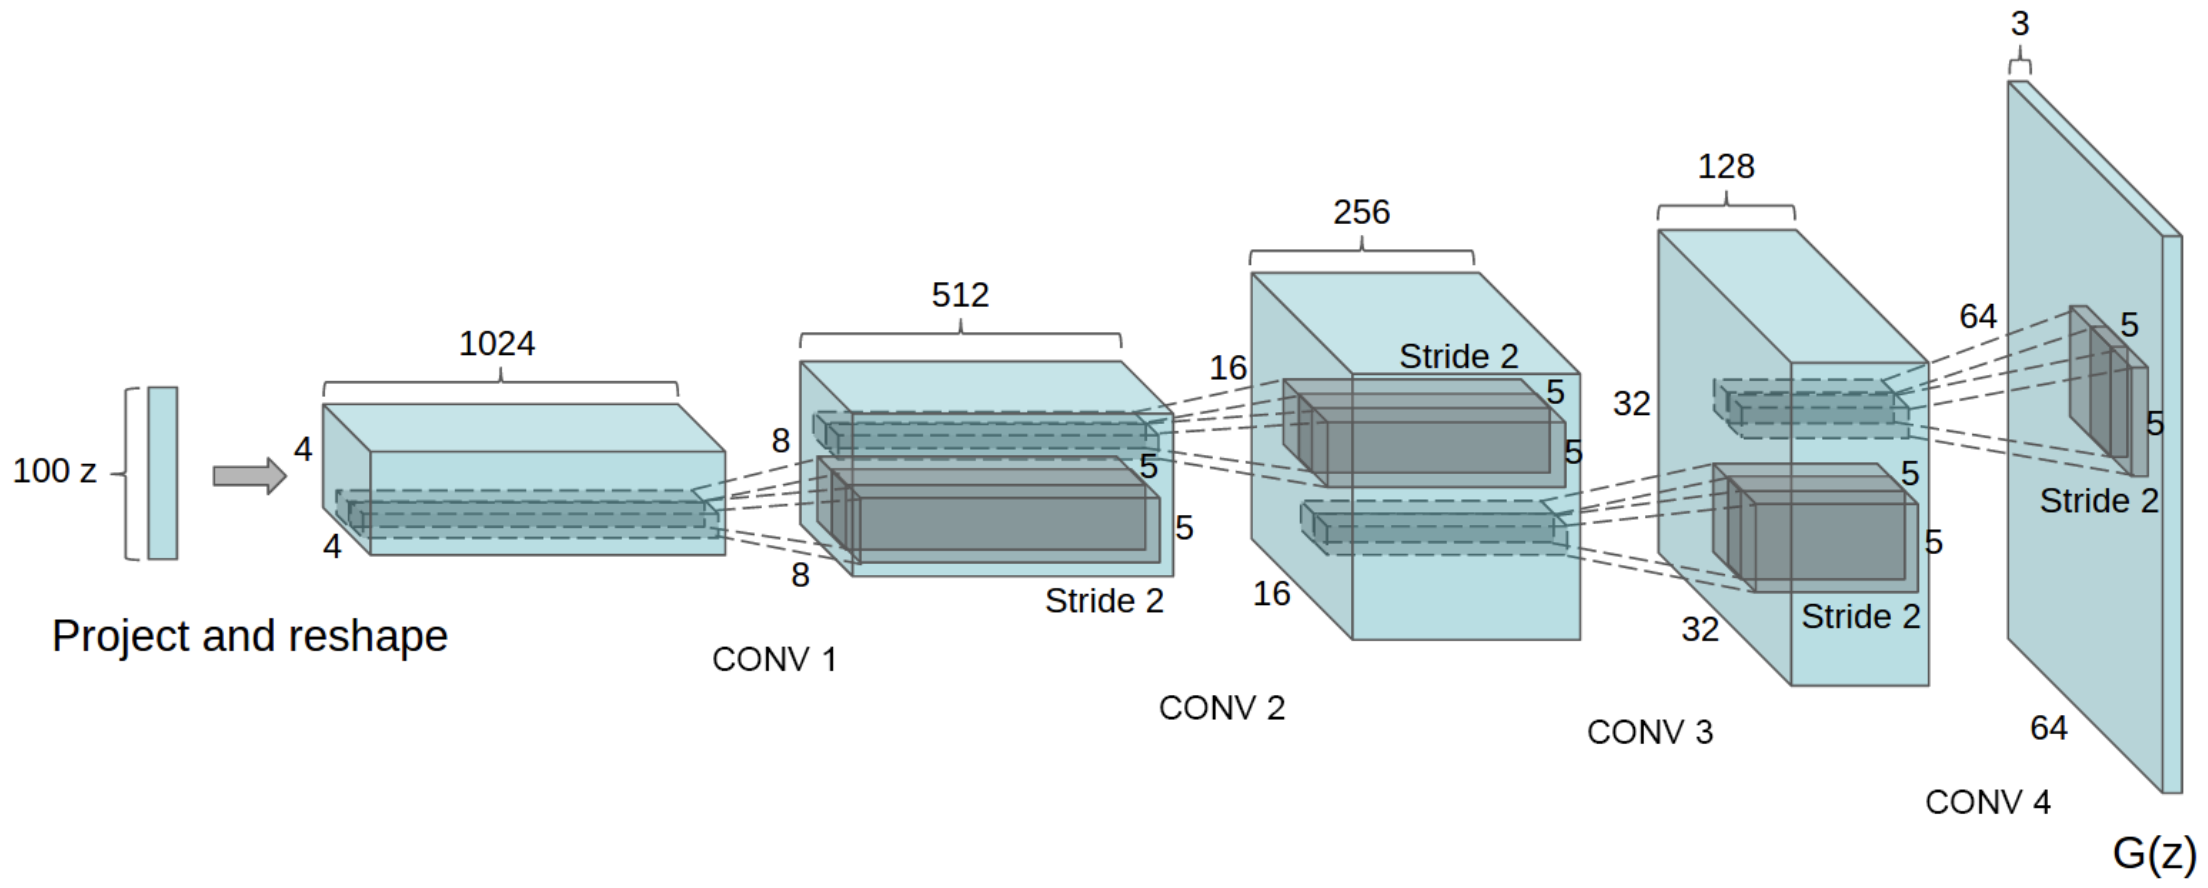
\includegraphics[width=0.8\linewidth]{figs/dcgan_1}
	\end{figure}
	\begin{itemize}
		\footnotesize
		\item  Mean-pooling instead of max-pooling.
		\item Transposed convolutions in the generator for upsampling.
		\item Downsample with strided convolutions and average pooling.
		\item ReLU for generator, Leaky-ReLU (0.2) for discriminator.
		\item Output nonlinearity: tanh for Generator, sigmoid for discriminator.
		\item Batch Normalization used to prevent mode collapse (not applied at the output of $G$ and input of $D$).
		\item Adam: small LR = 2e-4; small momentum: 0.5, batch-size: 128.
	\end{itemize}
	\myfootnotewithlink{https://arxiv.org/abs/1511.06434}{Radford A., Metz L., Chintala S. Unsupervised Representation Learning with Deep Convolutional Generative Adversarial Networks, 2015}
\end{frame}
%=======
\begin{frame}{Deep Convolutional GAN}
	\begin{block}{ImageNet samples}
		\begin{figure}
			\centering
			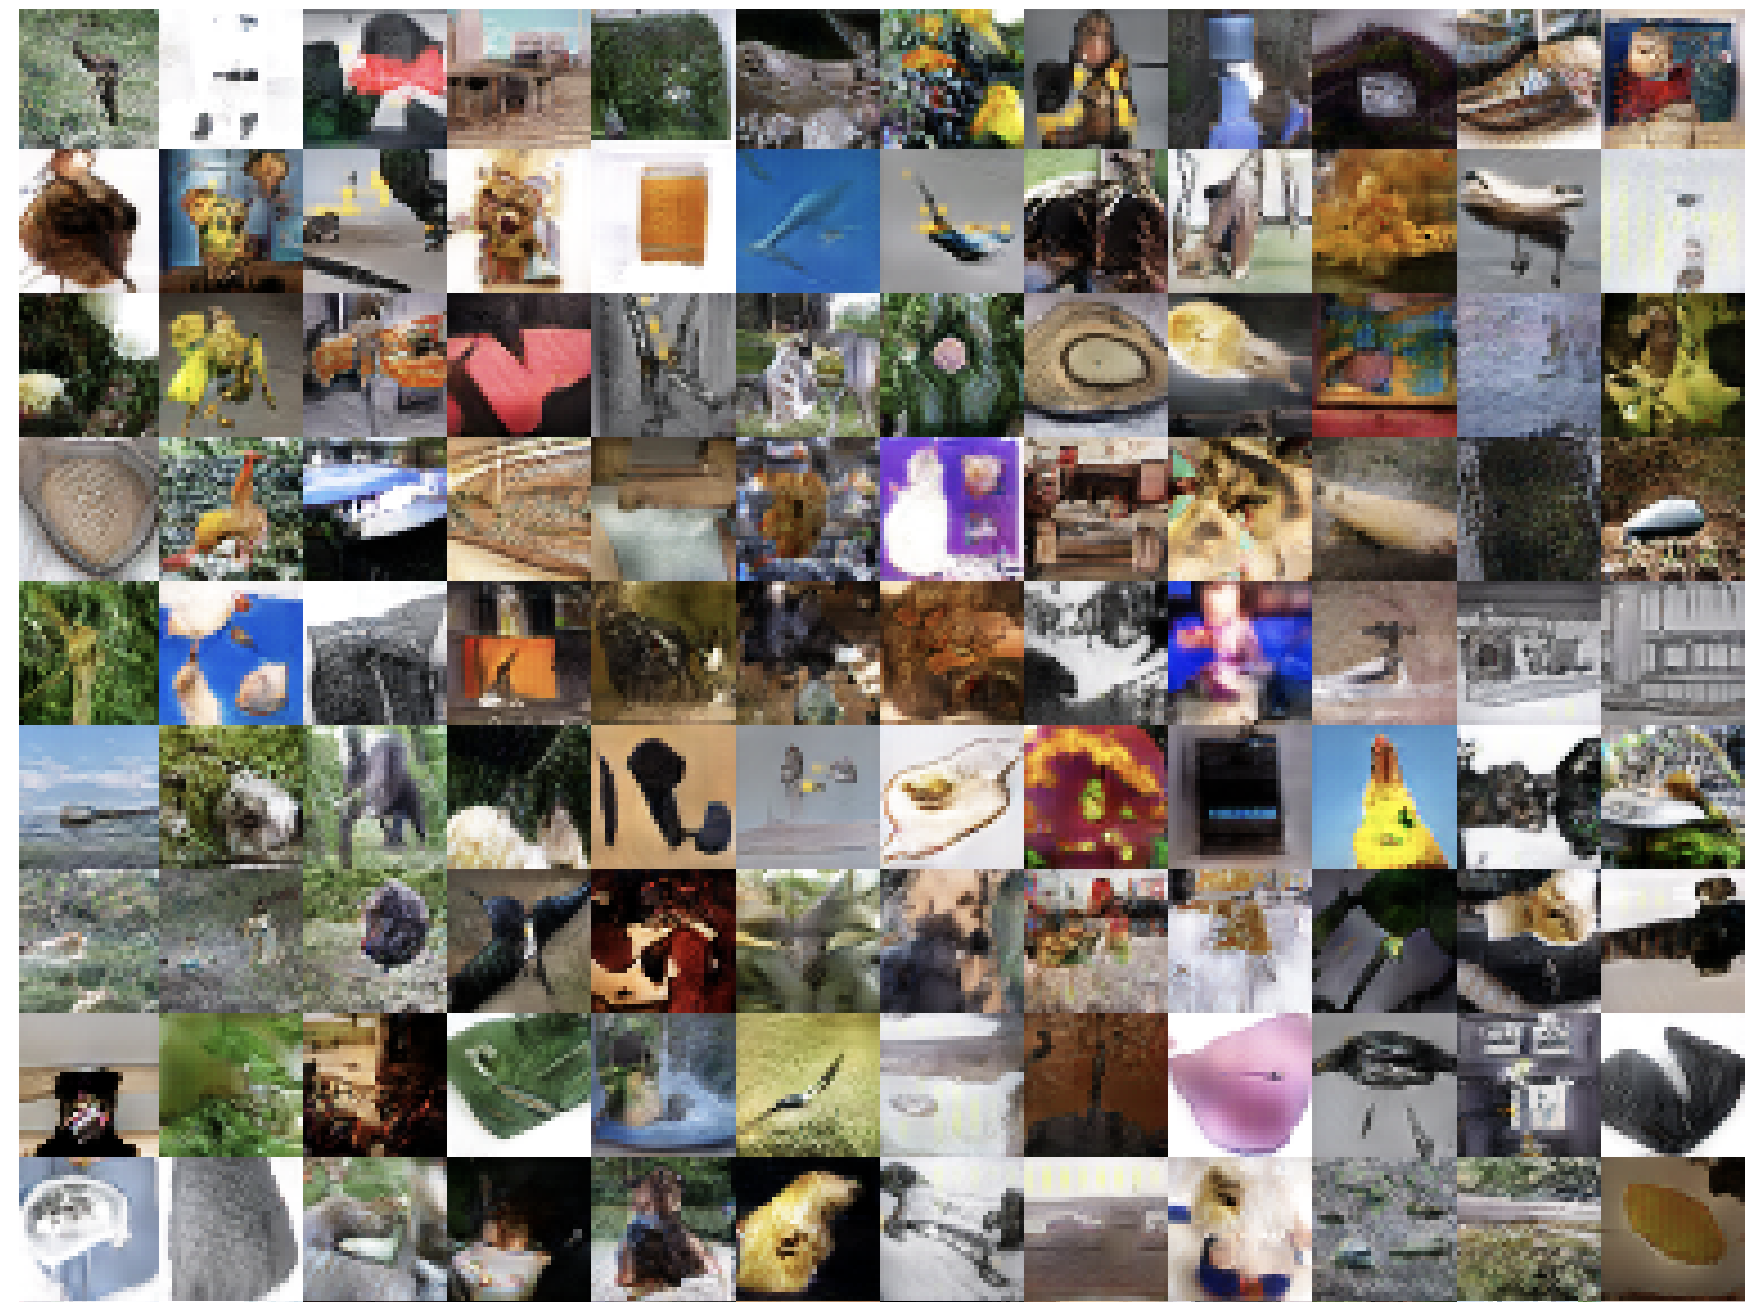
\includegraphics[width=0.8\linewidth]{figs/dcgan_results_1}
		\end{figure}
	\end{block}
	\myfootnotewithlink{https://arxiv.org/abs/1511.06434}{Radford A., Metz L., Chintala S. Unsupervised Representation Learning with Deep Convolutional Generative Adversarial Networks, 2015}
\end{frame}
%=======
\begin{frame}{Deep Convolutional GAN}
	\begin{block}{Smooth interpolations}
		\begin{figure}
			\centering
			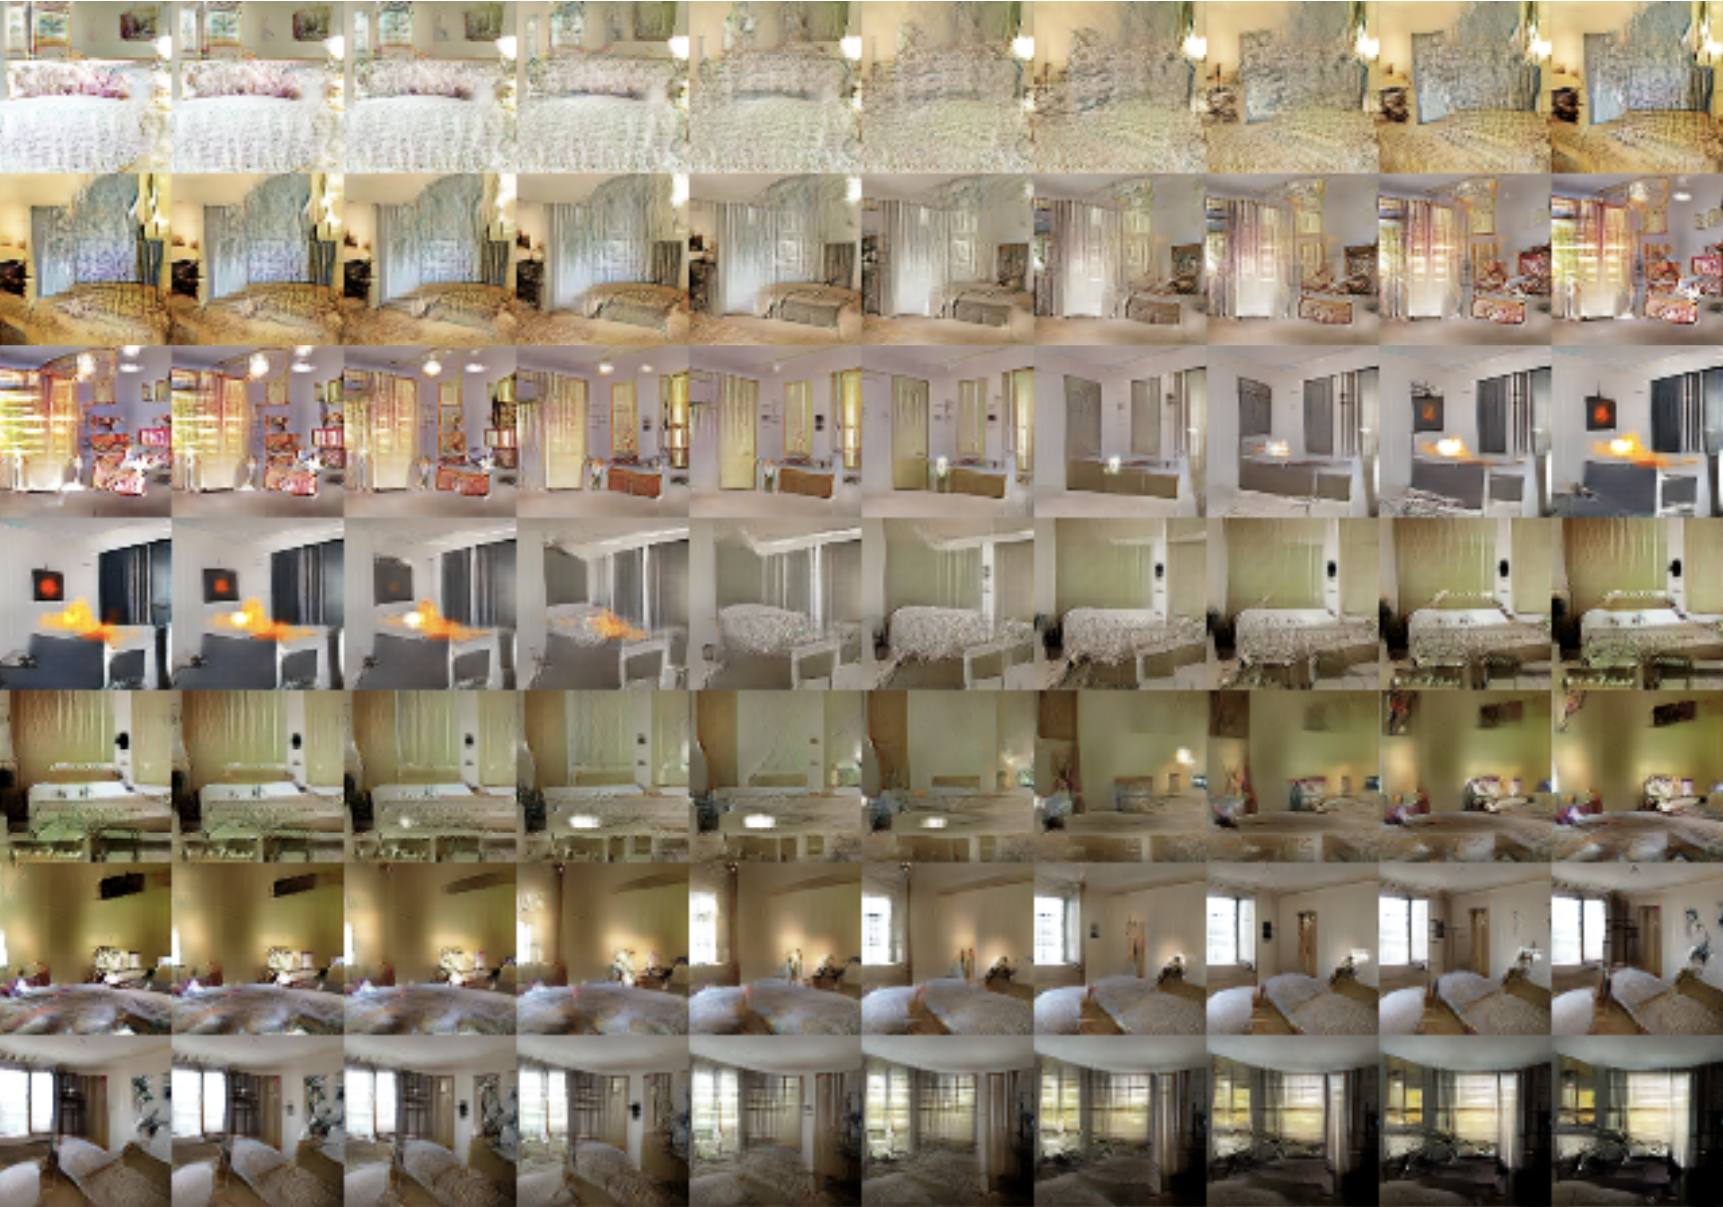
\includegraphics[width=0.8\linewidth]{figs/dcgan_results_2}
		\end{figure}
	\end{block}

	\myfootnotewithlink{https://arxiv.org/abs/1511.06434}{Radford A., Metz L., Chintala S. Unsupervised Representation Learning with Deep Convolutional Generative Adversarial Networks, 2015}
\end{frame}
%=======
\begin{frame}{Deep Convolutional GAN}
	\begin{block}{Vector arithmetic}
		\begin{figure}
			\centering
			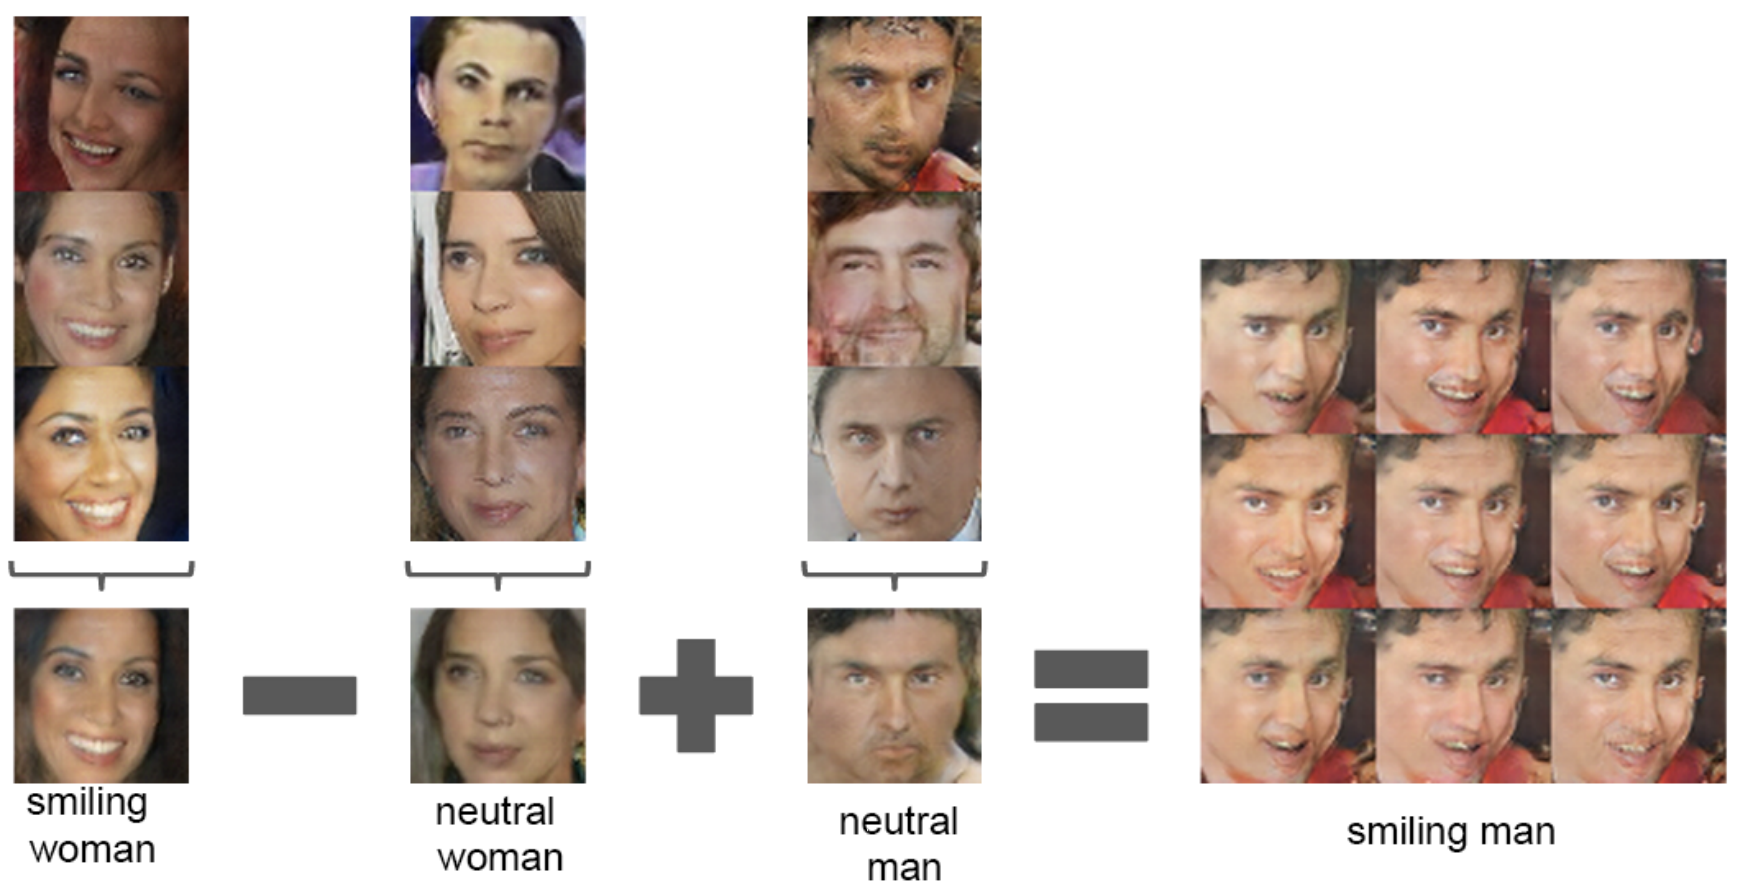
\includegraphics[width=1.0\linewidth]{figs/dcgan_results_3}
		\end{figure}
	\end{block}

	\myfootnotewithlink{https://arxiv.org/abs/1511.06434}{Radford A., Metz L., Chintala S. Unsupervised Representation Learning with Deep Convolutional Generative Adversarial Networks, 2015}
\end{frame}
%=======
\begin{frame}{Deep Convolutional GAN}
	\begin{block}{Mode collapse}
		\begin{figure}
			\centering
			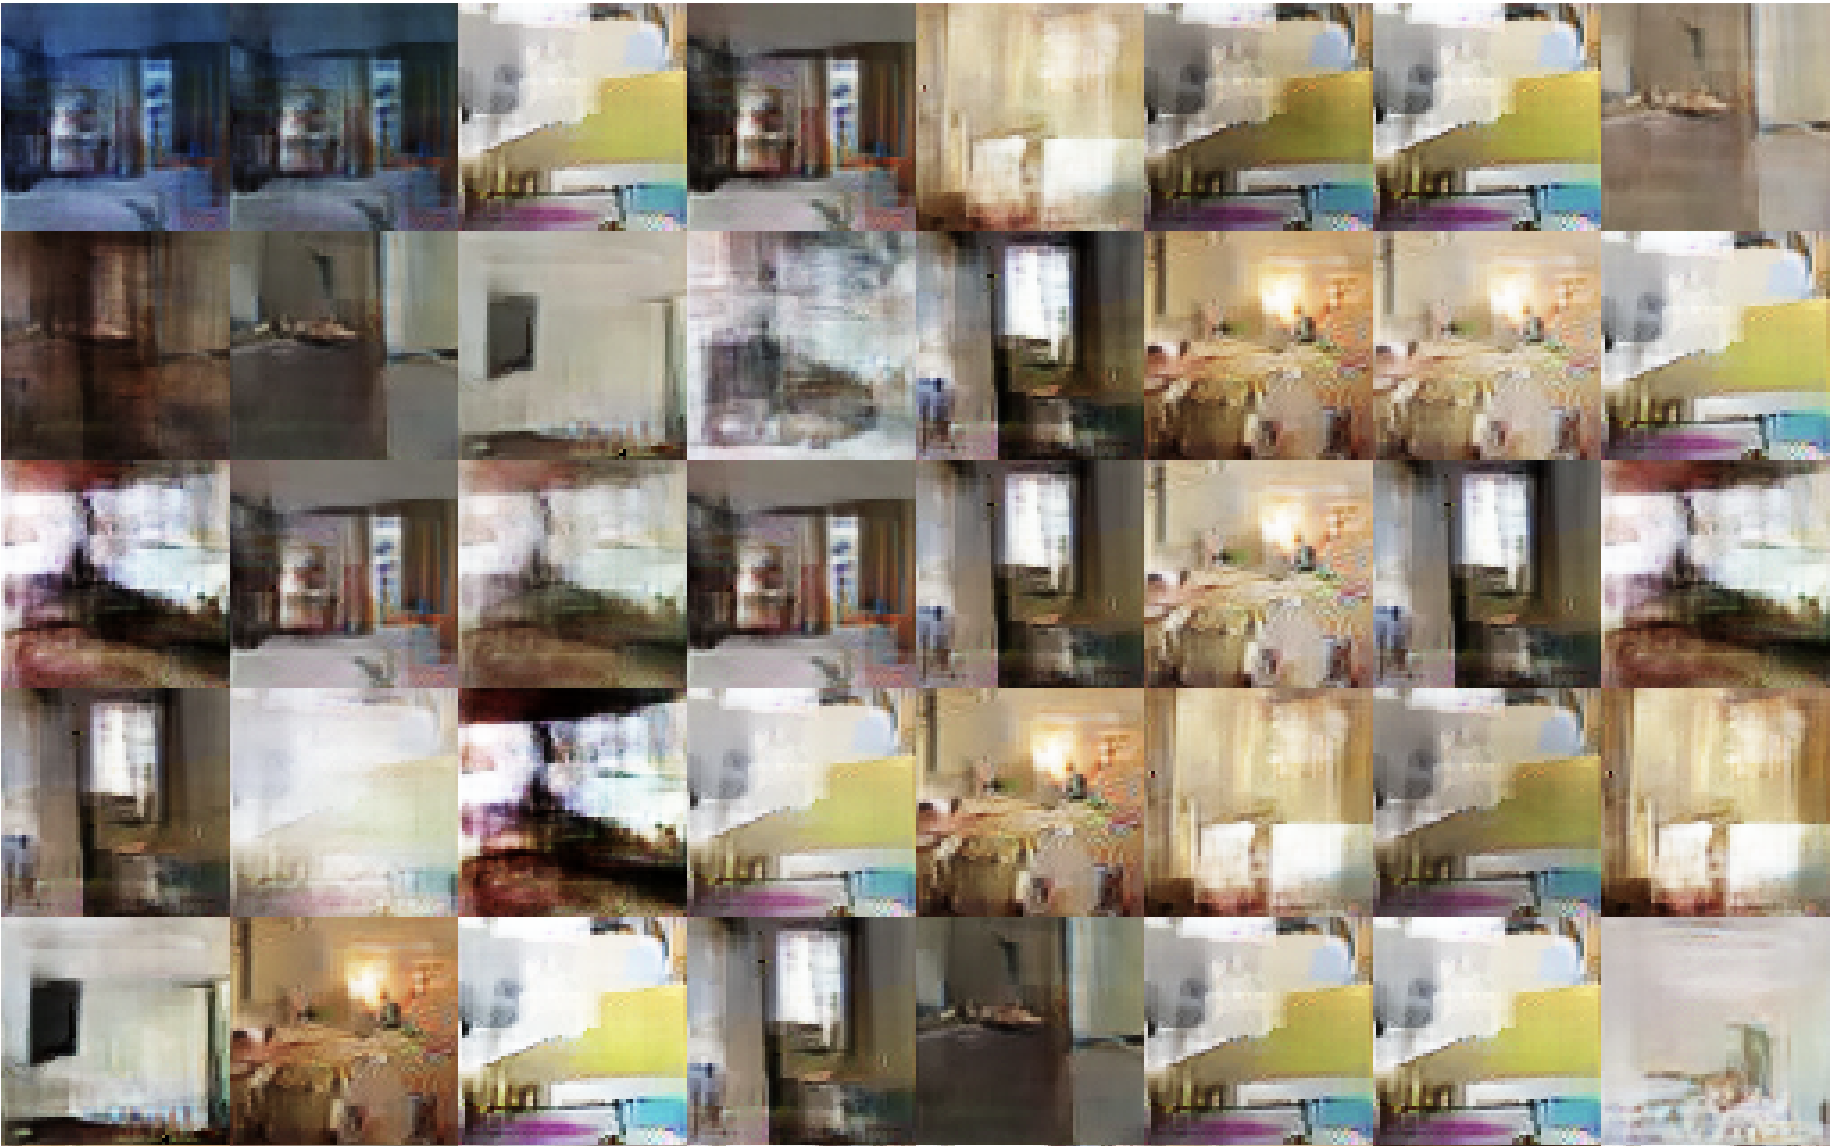
\includegraphics[width=0.95\linewidth]{figs/mode_collapse_4}
		\end{figure}
	\end{block}
	\myfootnotewithlink{https://arxiv.org/abs/1701.07875}{Arjovsky M., Chintala S., Bottou L. Wasserstein GAN, 2017}
\end{frame}
%=======
\begin{frame}{Summary}
	\begin{itemize}
		\item Majority of disentanglement learning models use heuristic objective or regularizers to achieve the goal, but the task itself could not be solved without good inductive bias.
		\vfill
		\item Likelihood is not a perfect criteria to measure quality of generative model.
		\vfill
		\item Adversarial learning suggest to solve minimax problem to match the distributions.
		\vfill
		\item Vanilla GAN tries to optimize Jensen-Shannon divergence (in theory).
		\vfill
		\item Mode collapse and vanishing gradients are the two main problems of vanilla GAN.
		\vfill
		\item Lots of tips and tricks has to be used to make the GAN training is stable and scalable.
	\end{itemize}
\end{frame}
%=======
\end{document} 